\documentclass[12pt]{article}
\usepackage{geometry}
\geometry{a4paper,left=1in,right=1in,top=1.3in,bottom=1.3in}
\usepackage{hyperref}
\usepackage{amsmath,amssymb,amsthm}
\usepackage{lipsum}
\usepackage{booktabs}
\usepackage{float}
\usepackage{graphicx}
\usepackage{xcolor}
\usepackage{fancyhdr}
\usepackage{url}
\usepackage{enumerate}
\usepackage{setspace}
\usepackage{amstext}
\usepackage{wrapfig}
\usepackage{indentfirst}
\usepackage{fontspec}
\usepackage[title]{appendix}
\usepackage[sorting=none]{biblatex}
\usepackage[ruled,linesnumbered]{algorithm2e}
\usepackage{subfigure}
\usepackage[table,xcdraw]{xcolor}


\setmainfont{Times New Roman}
\numberwithin{figure}{section}

\hypersetup{colorlinks=true,linkcolor=black,citecolor=red}    
\renewcommand{\baselinestretch}{1.2}
\newcommand{\setParDis}{\setlength {\parskip} {0.20cm} }


\newtheorem{theorem}{Theorem}
\newtheorem{corollary}[theorem]{Corollary}
\newtheorem{lemma}[theorem]{Lemma}
\newtheorem{definition}{Definition}

\addbibresource{main.bib}

\title{School Shootings in the U.S.: A Statistical Examination of Influencing Factors}

\author{Beijie Liu, Jingyan Zhang, Xinlei Cai}
\date{December 12, 2023}

\begin{document}

\maketitle

\section{Introduction}

According to \textcite{report}, school shootings have emerged as a grave concern, casting a dark shadow over educational institutions globally. These tragic events not only claim innocent lives but also instill a pervasive sense of insecurity and fear. The aftermath echoes through communities, affecting mental health, societal harmony, and the overall learning environment. The urgency to address this issue is underscored by its escalating frequency and the devastating impact on victims, families, and communities at large.

A plethora of research has been conducted to unravel the underlying causes and potential preventive measures for school shootings. While factors such as mental health, access to firearms, and school security have been extensively studied, there exists a noticeable gap in understanding the intricate role of socioeconomic factors. The complexity and multifaceted nature of these incidents necessitate a comprehensive exploration beyond the commonly examined variables, prompting a need to delve into the socioeconomic dimensions.

In this study, we aim to bridge this gap by meticulously examining specific indicators in different shooting incidences. The occurrence and severity of school shootings will be measured quantitatively, incorporating variables such as the frequency of incidents and the number of victims. This multifaceted approach ensures a comprehensive analysis, offering nuanced insights into the correlations and underlying patterns.

The central research question of this study seeks to unravel the correlation between different shooting factors and the occurrence and severity of school shootings. This inquiry is not only academic but also instrumental in shaping informed, targeted, and effective policy-making and prevention strategies. By unveiling the intricate relationships and contributing factors, the findings of this study aspire to inform robust strategies to preemptively mitigate the occurrence of school shootings and minimize their devastating impacts.

In the following part, we aims make use of three statistical methods, Welch’s permutation t-test, Monte Carlo Hypothesis Testing and linear regression to explore whether and how numerous factors affect the severity of school shootings. We will firstly make simulations and test the effectiveness of our strategies on different distribution of data (e.g. normal, right-skewed or linear). After figuring out the condition and assumptions of certain methods, we continue to perform analysis on real shooting data. Finally, we will make inference and possibly give reliable suggestions on school shooting prevention.

\section{Data}

The data used in this project were primarily sourced from \textcite{database} at the Naval Postgraduate School. Specifically, we relied on a recently released and comprehensive database of school shootings. This database aims to catalog every instance in which a firearm was brandished on school property, irrespective of the number of victims, the circumstances, or the time period. The database covers the period from 1970 to 2020.

\subsection{Data Preprocessing}

In the data preprocessing phase of this project, the primary focus was on ensuring the data's quality and suitability for analysis. The main steps involved in data preprocessing are summarized as follows:

\begin{itemize}
    \item Handling Missing Data:

    The dataset was checked for missing values (NA or unknown). Instances with missing values in key variables were either removed.

    \item Data Transformation:

    For instance, categorical variables were appropriately encoded into dummy variables.

    \item Outlier Detection and Treatment

    Outliers in the dataset were identified and assessed for their impact on the analysis. Depending on the context, outliers may have been removed
    
\end{itemize}

\subsection{Exploratory Data Analysis}

After cleaning data, we perform exploratory data analysis by drawing basic plots, showing graphical relationship between potential variables and number of injuries per shooting incidence. In the following part, we will show how to identify potential variables that could impact number of injuries per school shooting by two examples.

\begin{figure}[H]
    \centering
    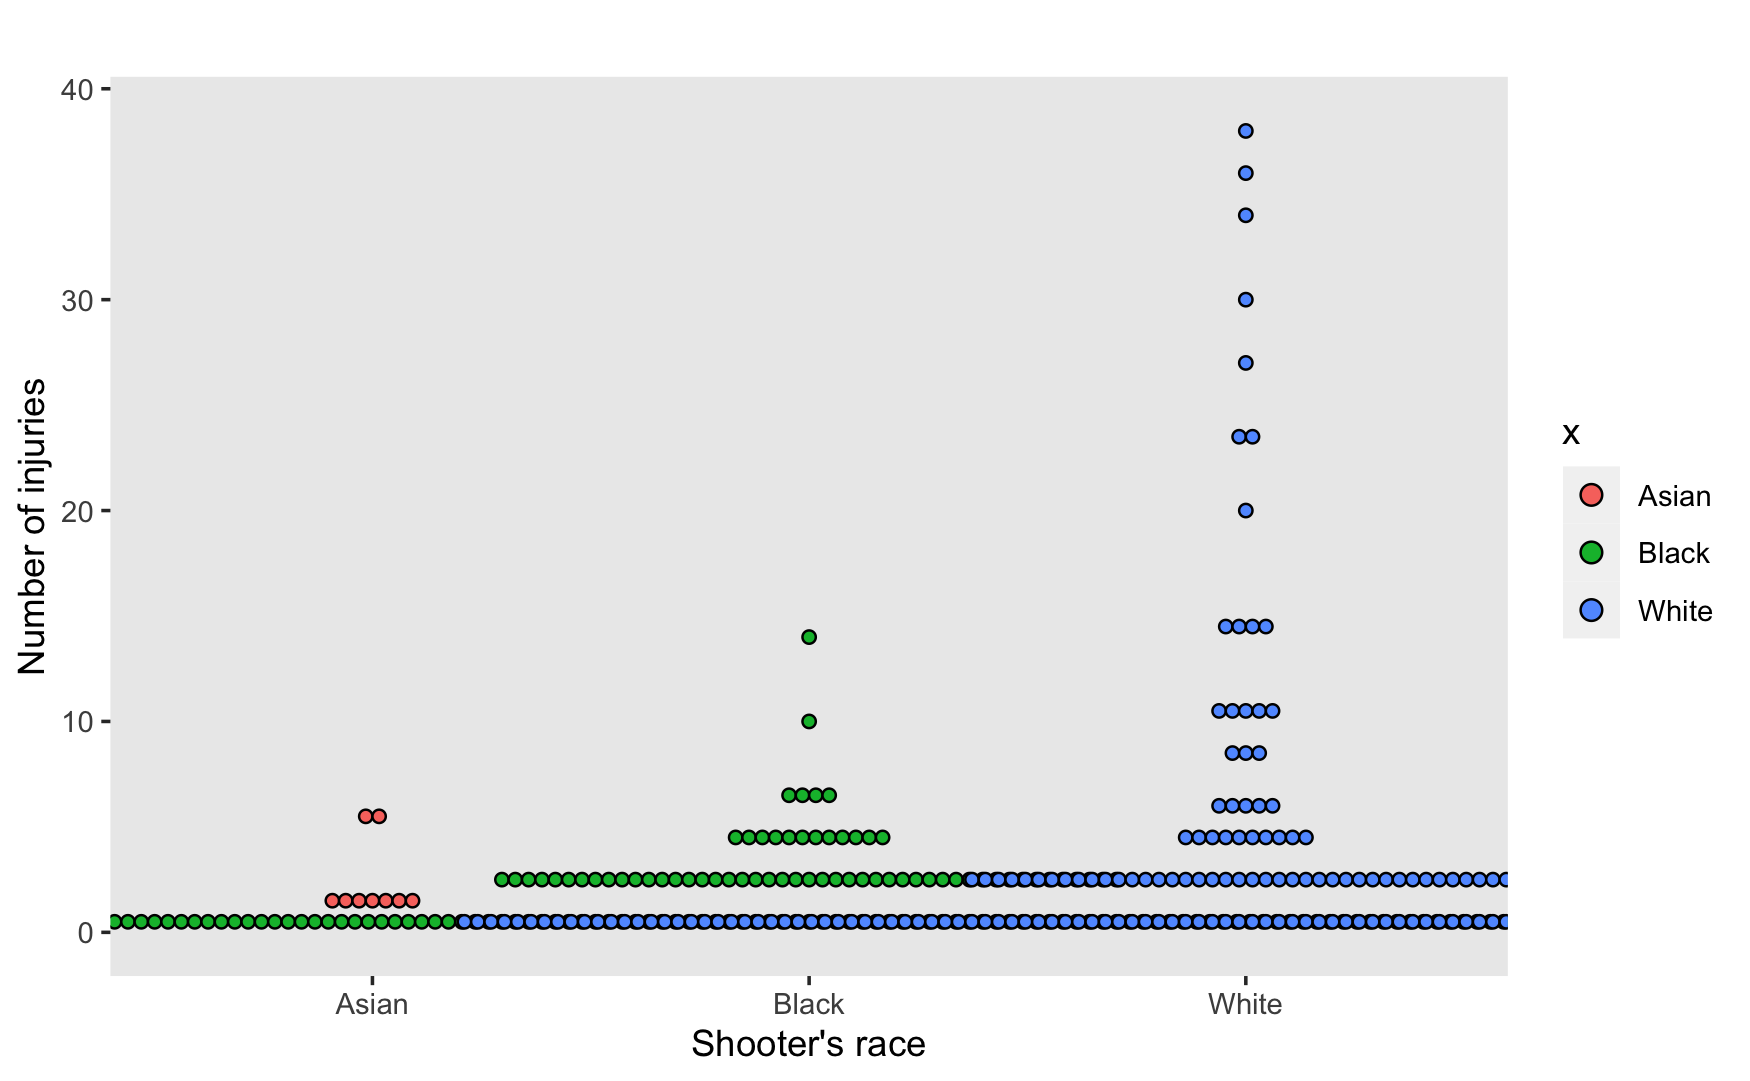
\includegraphics[width=0.8\textwidth]{explore_race.png}
    \caption{Dot plot showing number of injuries among different shooter's races}
    \label{explore_race}
\end{figure}

By drawing dot plots, we can tell whether there is a difference in injuries among different races of shooters. From \ref{explore_race}, there is a clear pattern shows that white shooters are likely to cause injuries.

\begin{figure}[H]
    \centering
    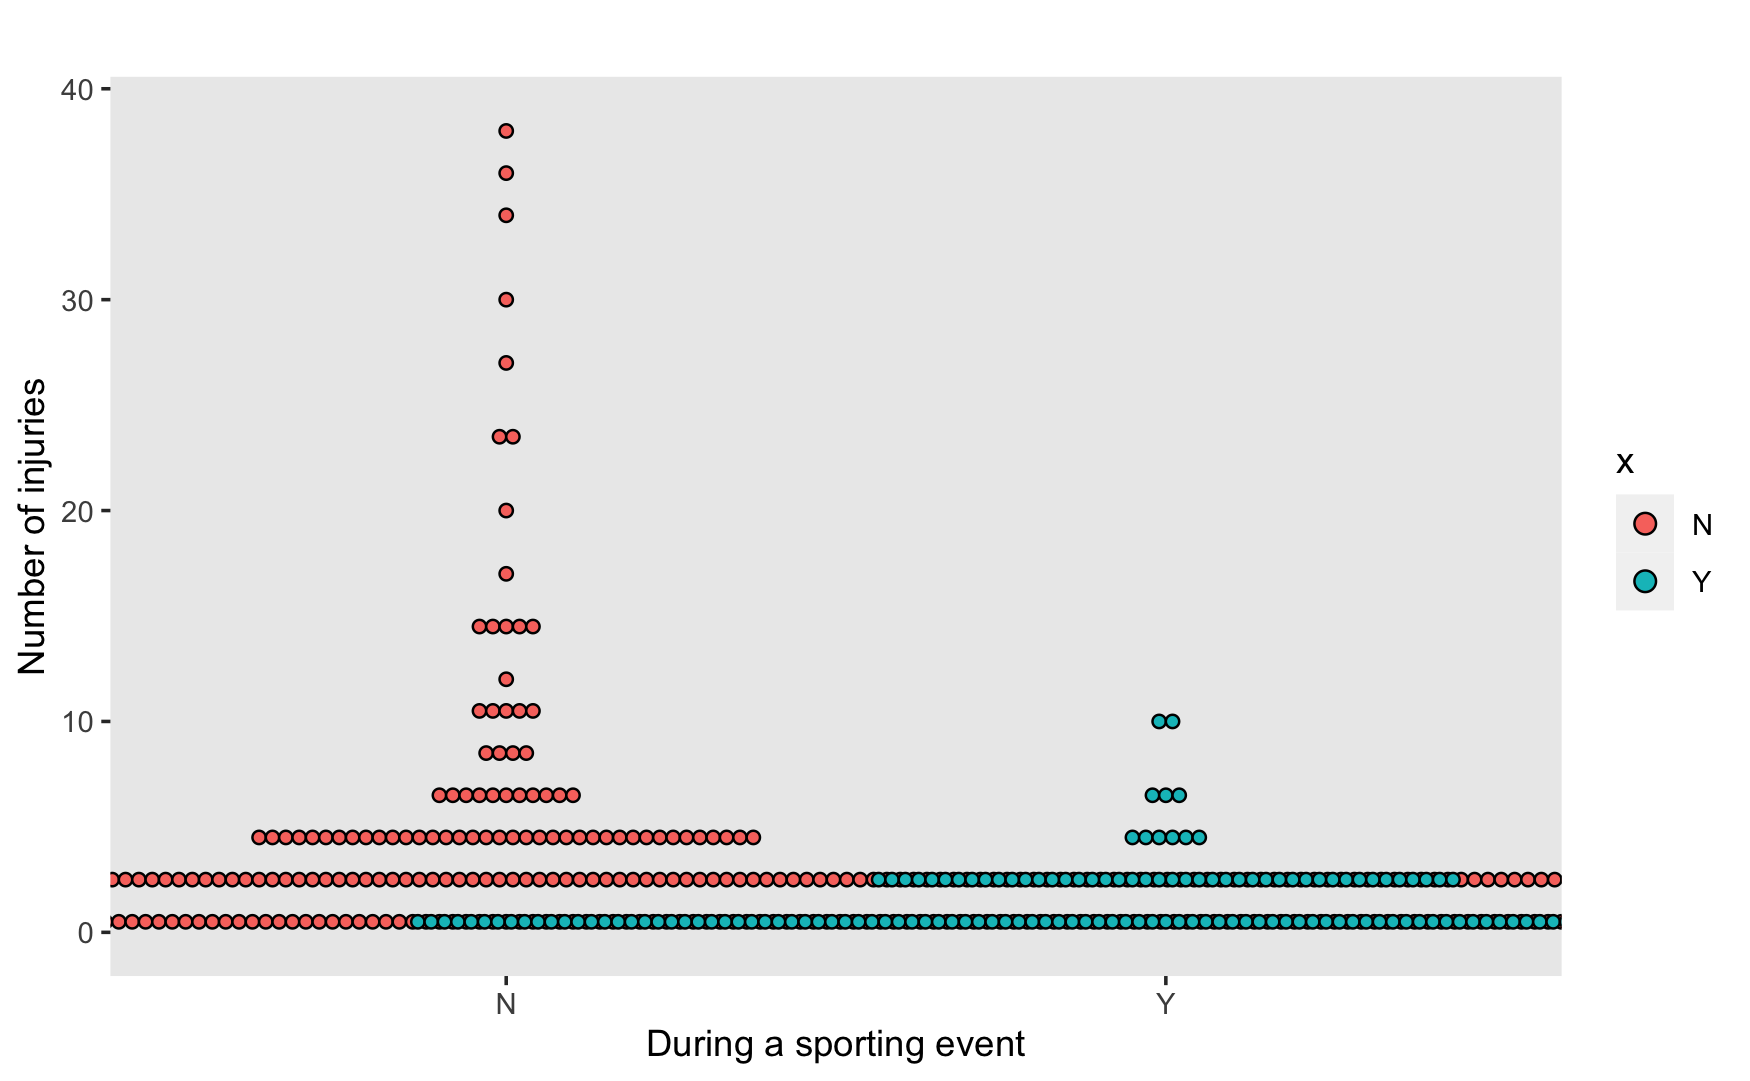
\includegraphics[width=0.8\textwidth]{explore_sports.png}
    \caption{Dot plot showing number of injuries during sports events or not}
    \label{explore_sports}
\end{figure}

Similarly, we draw dot plots between injuries and whether shooting occurs during a sporting event. \ref{explore_sports} indicates that shootings that cause large injuries tend not to happen during sports.

By carrying out exploratory data analysis through graphs, we manage to grasp an initial feeling in the research question. Note that graphical inference is not precise. It only provides a foundation for our research question.

\subsection{Key Variables}

After data cleaning and exploratory analysis, we find some key variables form the basis of our analysis, allowing us to examine patterns, trends, and factors associated with school shootings over the specified time frame. 

\begin{itemize}
    \item Number of Injuries
    \item Categorization
    \item Time and Day of the Week
    \item Firearm Involvement
    \item Shooter and Victim Demographics
    \item Shooter's Past Experience
\end{itemize}


\section{Method}

We aim to apply three statistical methods to explore the relationship between shooting injuries and other features. In this part, we will describe in sufficient detail the method for analysis, state the assumptions the method requires, and discuss the computational aspects of the approach.

\subsection{Welch's permutation t-test}

Welch's permutation t-test is a statistical method that merges the principles of Welch's t-test and permutation testing, offering a robust solution for comparing two groups with unequal variances and sample sizes. This test modifies Welch's t-test, which adjusts for unequal variances, by incorporating permutation techniques to generate the distribution of the test statistic without relying on standard distributional assumptions. 

Welch's permutation t-test will compare the means of two independent groups (e.g., male shooters vs. female shooters) to see if there is a statistically significant difference in the number of injuries. According to \textcite{slides_perm}, the process of Welch's permutation test is:

\begin{itemize}
    \item Calculate the mean difference between the two groups.
    \item Randomly permute the labels (gender) of the data points and recalculate the mean difference for these permuted samples.
    \item Repeat the permutation process a large number of times (e.g., 10,000 times) to create a distribution of mean differences.
    \item Determine where the actual observed mean difference falls within this distribution.
\end{itemize}

Welch's permutation t-test operates on several key assumptions. Firstly, it assumes the independence of observations, meaning each school shooting incident in the dataset should be independent of the others. Our dataset agrees with this requirement this we can safely assume no relationship between each school shooting incidence. Secondly, while it is less sensitive to the normality assumption compared to other t-tests, it generally assumes that the distributions of the groups being compared are roughly symmetric. Note that our real dataset is not guaranteed to be symmetric distributed. So we will test the effectiveness of the method on less symmetric data (e.g., right skewed normal distribution). Thirdly, unlike the standard t-test, Welch's test does not assume equal variances across groups, making it suitable for datasets where this assumption might be violated. This flexibility in handling unequal variances is particularly advantageous in real-world data scenarios like school shooting analyses, where data distributions can vary significantly between groups. Finally, it is admitted that this method is typically used to compare two groups. If some features have multiple categories, it is hard to implement this method to reveal the difference for each group. We inspect our dataset and find that many of the features are binary (e.g., Y/N condition). Therefore, with respect to these features, we can confidently use this method.

The computational aspect of Welch's permutation t-test involves handling potentially large datasets and executing numerous permutations, which demands efficient computational strategies. This necessitates the use of powerful statistical software or programming languages like R, equipped with specialized libraries for data analysis and permutation testing. The process includes generating a large number of permutations to create a robust empirical distribution of mean differences under the null hypothesis. In our research, we choose to use some standard library and function in R to speed up the process. Besides, the dataset we use the dataset containing incidences of school shooting from 1970 to 2020 (about 1500 cases), which is comparatively small in statistical consideration. Therefore, Welch's permutation t-test fits for our research. 

\subsection{Monte Carlo Hypothesis Testing}

Monte Carlo hypothesis testing is a powerful statistical technique used to assess hypotheses and make inferences about population parameters. It is particularly useful when analytical solutions are challenging or impossible to obtain. This method involves simulating random data under specific assumptions and comparing the observed results with the simulated ones to make statistical inferences.

According to \textcite{slides_mc}, the general process of Monte Carlo hypothesis testing can be summarized as follows:

\begin{enumerate}
    \item Formulate a null hypothesis ($H_0$) and an alternative hypothesis ($H_a$) to be tested.
    \item Define a test statistic that measures the effect or relationship of interest between variables.
    \item Collect observed data and calculate the observed test statistic.
    \item Simulate a large number of datasets under the null hypothesis or other specified conditions.
    \item Calculate the test statistic for each simulated dataset.
    \item Construct a distribution of test statistics based on the simulations.
    \item Compare the observed test statistic to the simulated distribution.
    \item Calculate a p-value representing the likelihood of observing results as extreme as, or more extreme than, the observed results under the null hypothesis.
    \item Make a decision about whether to reject or fail to reject the null hypothesis based on the p-value and a chosen significance level.
\end{enumerate}


Monte Carlo hypothesis testing operates under several key assumptions:

\begin{enumerate}
    \item \textbf{Independence of Observations}: The observations in the dataset should be independent, meaning that the outcome of one observation does not influence the outcome of another. This assumption is crucial to ensure the validity of the method.
    
    \item \textbf{Distributional Assumptions}: While Monte Carlo methods are less sensitive to distributional assumptions compared to traditional tests, they may still require certain distributional properties. The appropriateness of these assumptions depends on the specific test and simulation design.
    
    \item \textbf{Random Sampling}: Simulated datasets are typically generated through random sampling or permutations. The randomness of the sampling process is fundamental to the validity of Monte Carlo simulations.
\end{enumerate}

The computational aspects of Monte Carlo hypothesis testing can be demanding, especially when dealing with a large number of simulations or complex statistical models. Efficient programming languages and libraries are often employed to accelerate the process.

In practice, the computational steps involve generating numerous permutations or simulations, each requiring calculations of the test statistic. The computational efficiency can significantly impact the feasibility and speed of the analysis.

The method's foundations align with the principles of statistical hypothesis testing, including the use of p-values to quantify evidence against the null hypothesis. Monte Carlo simulations enable researchers to perform hypothesis tests in situations where exact analytical solutions may be unattainable, making it a valuable tool in modern statistical practice.

In the subsequent sections, we will explore linearity between predictors using Monte Carlo hypothesis testing.


\subsection{Linear Regression}
% Methodology
Least Squares is a cornerstone technique in statistical analysis, primarily used in linear regression to estimate the relationships between variables. This method focuses on minimizing the sum of the squared differences between observed values and those predicted by a linear model, thereby ensuring the best possible fit.

Linear regression is a robust statistical tool used for modeling the relationship between a dependent variable and one or more independent variables. In this context, the dependent variable is the count of total victims, and the independent variables are different properties of the school shooting incidents.

% Assumptions of the Method
According to \textcite{slides_lm}, the linear regression approach is underpinned by several key assumptions:

\begin{itemize}
    \item Linearity: The relationship between the independent variables (predictors) and the dependent variable (outcome) is linear.
    \item Independence: Observations are independent of each other. For instance, there is no correlation between the residuals (errors) of the observations.
    \item Homoscedasticity: The residuals have constant variance at every level of the independent variables. 
    \item Normality of Residuals: The residuals of the model are normally distributed. 
    \item No Multicollinearity: The independent variables are not too highly correlated with each other.
\end{itemize}

% Computational Aspects
Computationally, the model will be fitted using the Ordinary Least Squares (OLS) method, which minimizes the sum of the squared differences between observed and predicted values. This method is both computationally efficient and provides interpretable parameters, making it a standard choice for linear regression problems. We will utilize dummy variable coding to convert the categorical independent variable into a numerical format suitable for regression analysis.

% % Connection to Statistical Theory
% Our analytical approach is grounded in the classical linear regression framework, which provides a parametric means of modeling the relationship between variables. The regression coefficients estimated from this model will quantify the change in the total number of victims associated with each gender category of victims, after adjusting for other variables in the model. The significance of these coefficients will be determined using t-tests, with the underlying statistical theory providing both estimates of effect sizes and measures of uncertainty (p-values and confidence intervals).

In our study, we utilize linear regression analyzed through the Ordinary Least Squares (OLS) method, a widely accepted approach in statistics. The choice of OLS is underpinned by the Gauss-Markov Theorem, a fundamental principle that ensures the reliability of our estimates under certain conditions, such as a linear relationship between variables, independence of observations, and consistent variability. This theorem guarantees that, provided these conditions are met, the OLS method yields the most accurate and unbiased estimates for our linear model. Applying this to our context, where we examine the relationship between school shootings and victim counts, adhering to these conditions helps ensure that our analysis is both accurate and credible. The robustness of our methodology is further reinforced through stringent model validation techniques.

To ensure the validity of our model, we'll be using the R-squared statistic to assess its explanatory power, essentially measuring how much of the variability in victim counts can be explained by our chosen independent variables. We will rigorously validate the assumptions of our model using residual plots and various diagnostic tests. This step is crucial to ensure that our model accurately reflects the underlying data and theoretical assumptions. If we find that our model assumptions are violated, we are prepared to explore alternative specifications or apply transformation techniques. This process not only enhances the reliability of our findings but also ensures that our analysis remains grounded in robust statistical practices, seamlessly integrating theory with practical application.

\section{Simulation}

\subsection{Welch’s permutation t-test}

In this part, we generate data with three different types of distributions: normal, right-skewed normal, and left-skewed normal. This variation helps to assess the test's robustness to deviations from normality. In each kind of distribution, we keep one group unchanged and vary the mean and standard deviation of the other group and obtain p-value by Welch’s permutation t-test. Finally, we plot heat maps using R, where the x-axis represents the mean, the y-axis represents the standard deviation, and the color intensity indicates the p-value. Note that the two black dotted lines in each graph denotes the group with fixed mean and sd. This visual representation will illustrate the conditions under which the null hypothesis is rejected.

\begin{figure}[H]
    \centering
    \subfigure[Normal]{
        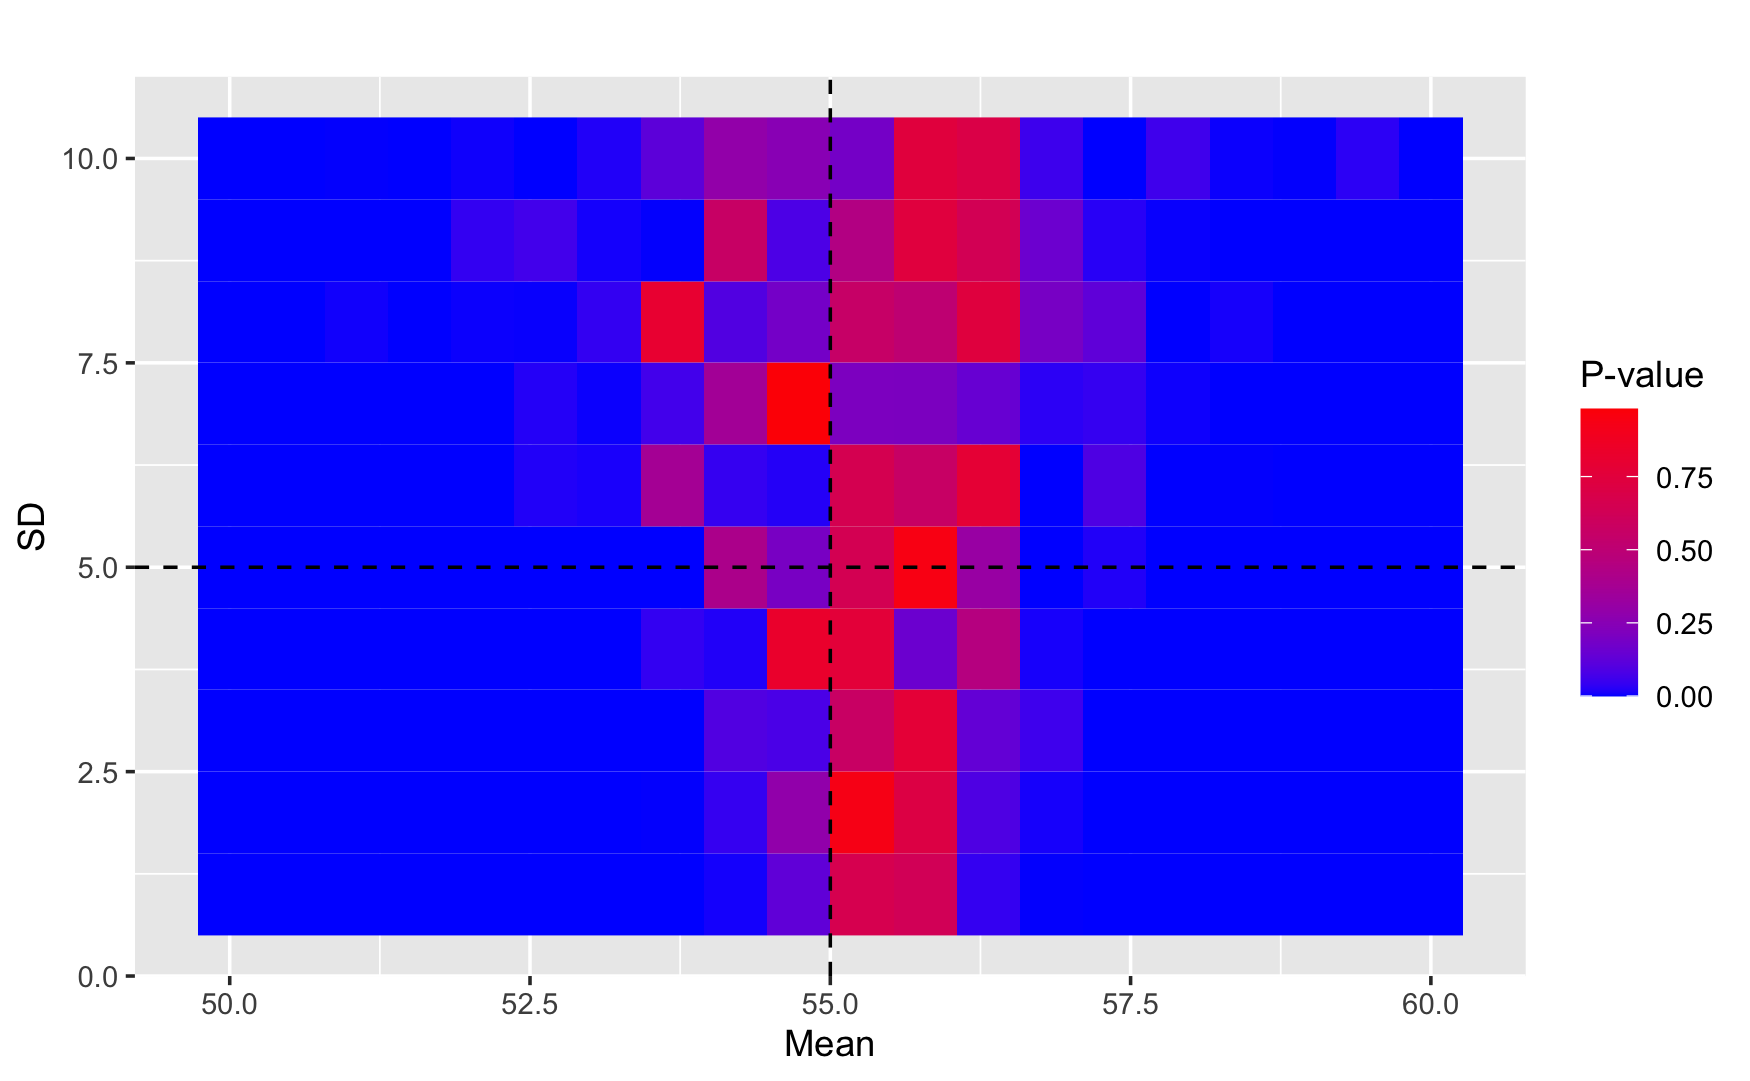
\includegraphics[width=0.3\textwidth]{permtest_heatmap_normal.png}
        \label{fig:heatmap_normal}
    }
    \subfigure[Left-skewed Normal]{
        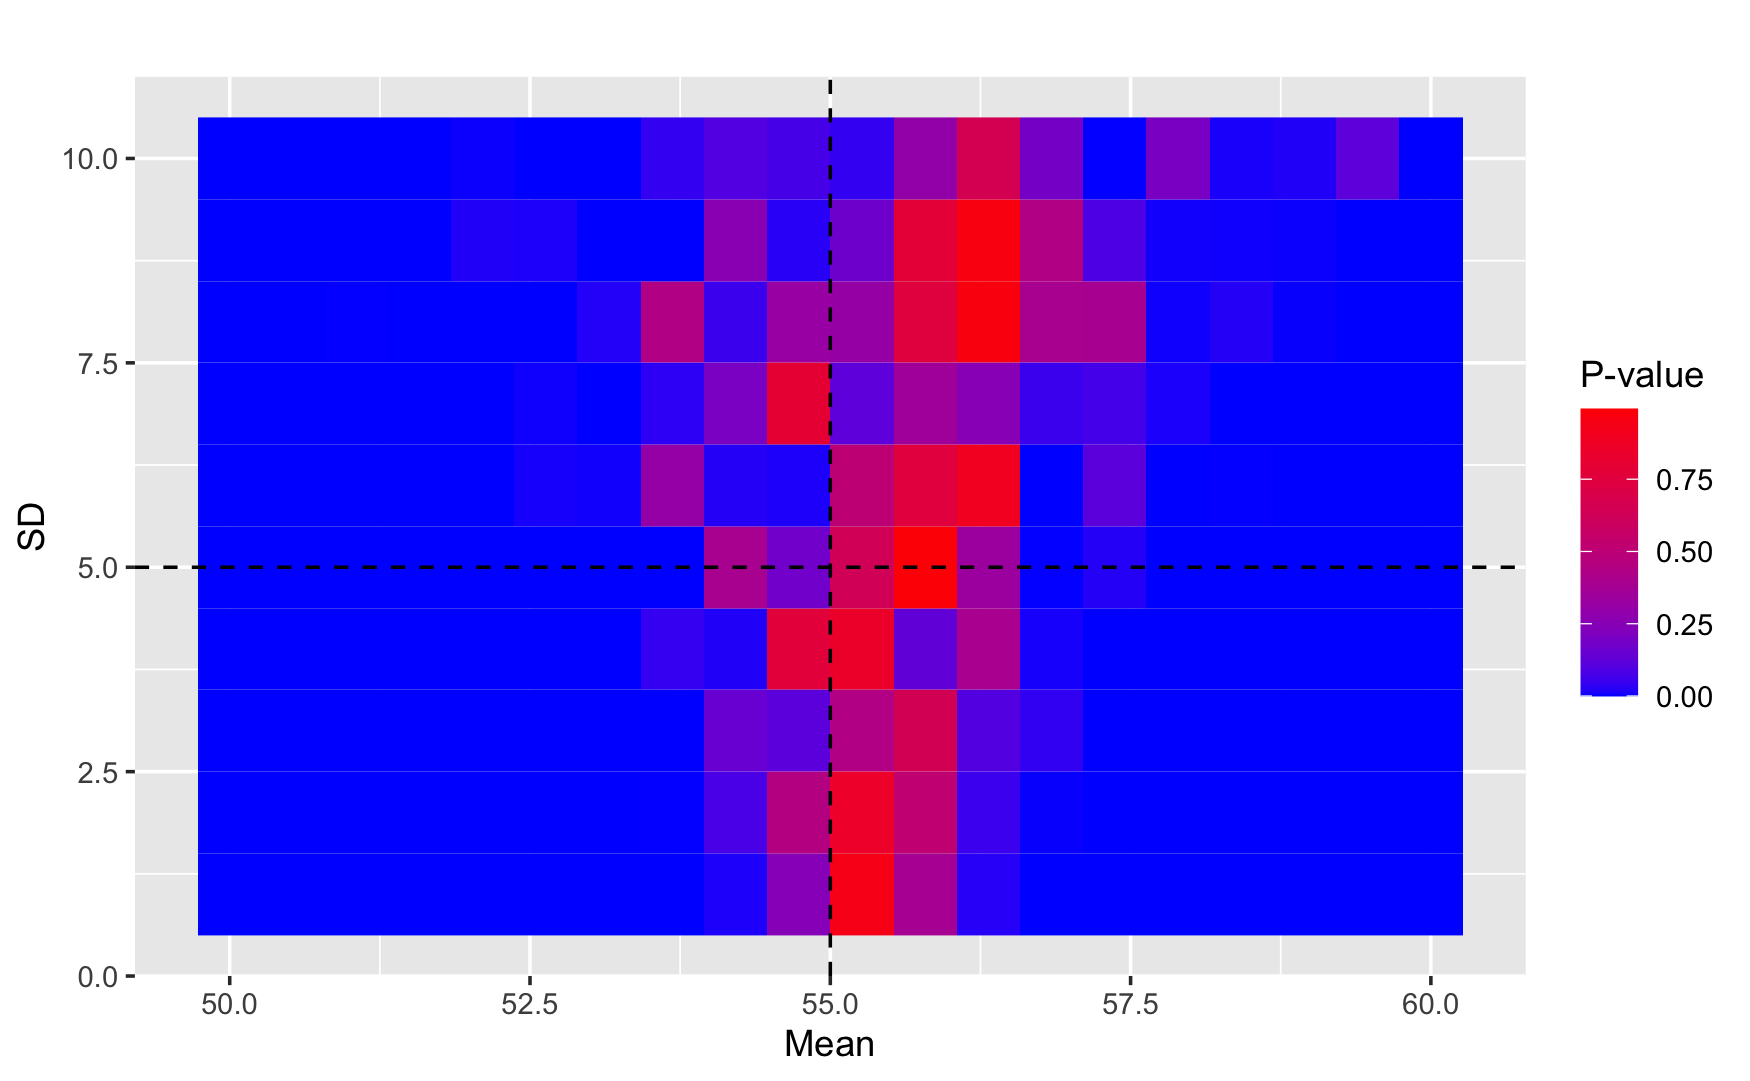
\includegraphics[width=0.3\textwidth]{permtest_heatmap_left.png}
        \label{fig:heatmap_left}
    }
    \subfigure[Right-skewed Normal]{
        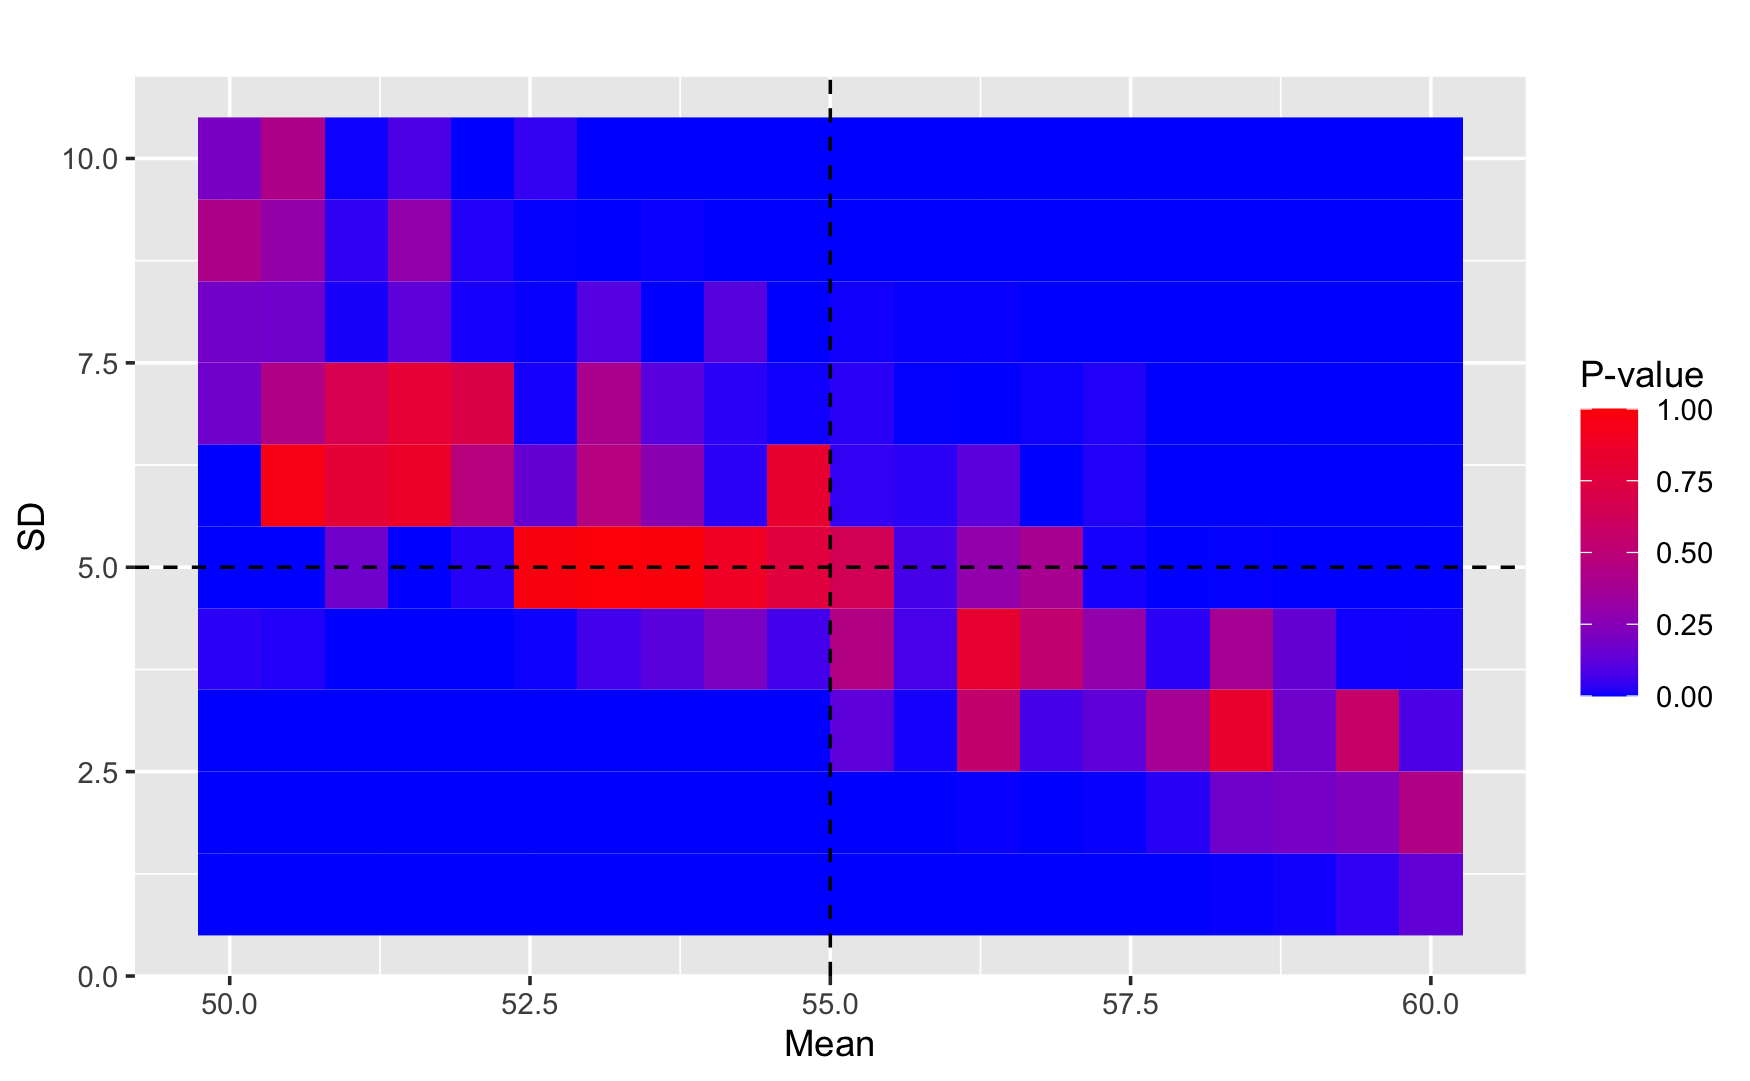
\includegraphics[width=0.3\textwidth]{permtest_heatmap_right.png}
        \label{fig:heatmap_right}
    }
    \caption{Comparative Heat Maps of the Simulation Results}
    \label{fig:heatmaps}
\end{figure}

From the simulation, we can conclude that for \ref{fig:heatmap_normal} and \ref{fig:heatmap_left}, Welch’s permutation t-test is sensitive even when the variance of two groups are quite different. It is worth mentioning that the performance is better when the variance of two groups are near. However, for the \ref{fig:heatmap_right}, the method fails to reject the null hypothesis even if their difference in mean is significant.

This fact indicates that if the real data is normal or left-skewed normal distributed, we can safely use Welch’s permutation t-test. If it follows right-skewed normal distribution, we might have to consider other methods.


\subsection{Monte Carlo Hypothesis Testing}

In this part, we generate data with different types of distribution and explore possible linear relationships between them. We use Monte Carlo Hypothesis Test that:
\begin{itemize}
    \item \textbf{Null hypothesis:} There is no linear relationship between two sets of data.
    \item \textbf{Alternative hypothesis:} There is linear relationship between two sets of data.
\end{itemize}
So we need to calculate Pearson's correlation coefficients to measure the linear correlation between two sets of data. Firstly, we use Monte Carlo techniques to draw samples from one data set and fix another. In each kind of distribution, we define the function to fix the first data set while sampling from the second data set. Then we calculate the simulated correlation based on samples. Compared with the observed correlation value that directly obtained from two sets of data, we get the two-tailed p-value. In our simulation, let $\alpha = 0.05$ is the significant level. If p-value is less than or equal to 0.05, we have strong confidence to reject the null hypothesis and consider there exists linear relationship between two data sets.

To generate the data, we fix Group A data set with mean=0 and standard deviation=1 in first three experiment, min=3 and max=7 in Uniform distribution. Group B are generated by a sequence of means and standard deviation in normal and right-skewed normal distribution; a sequence of lambda in exponential distribution; a sequence of minimum and maximum values. The visual representation of p-values are shown in Fig. \ref{4.2}.

\begin{figure}[H]
    \centering
    \subfigure[Normal v.s. Normal]{
       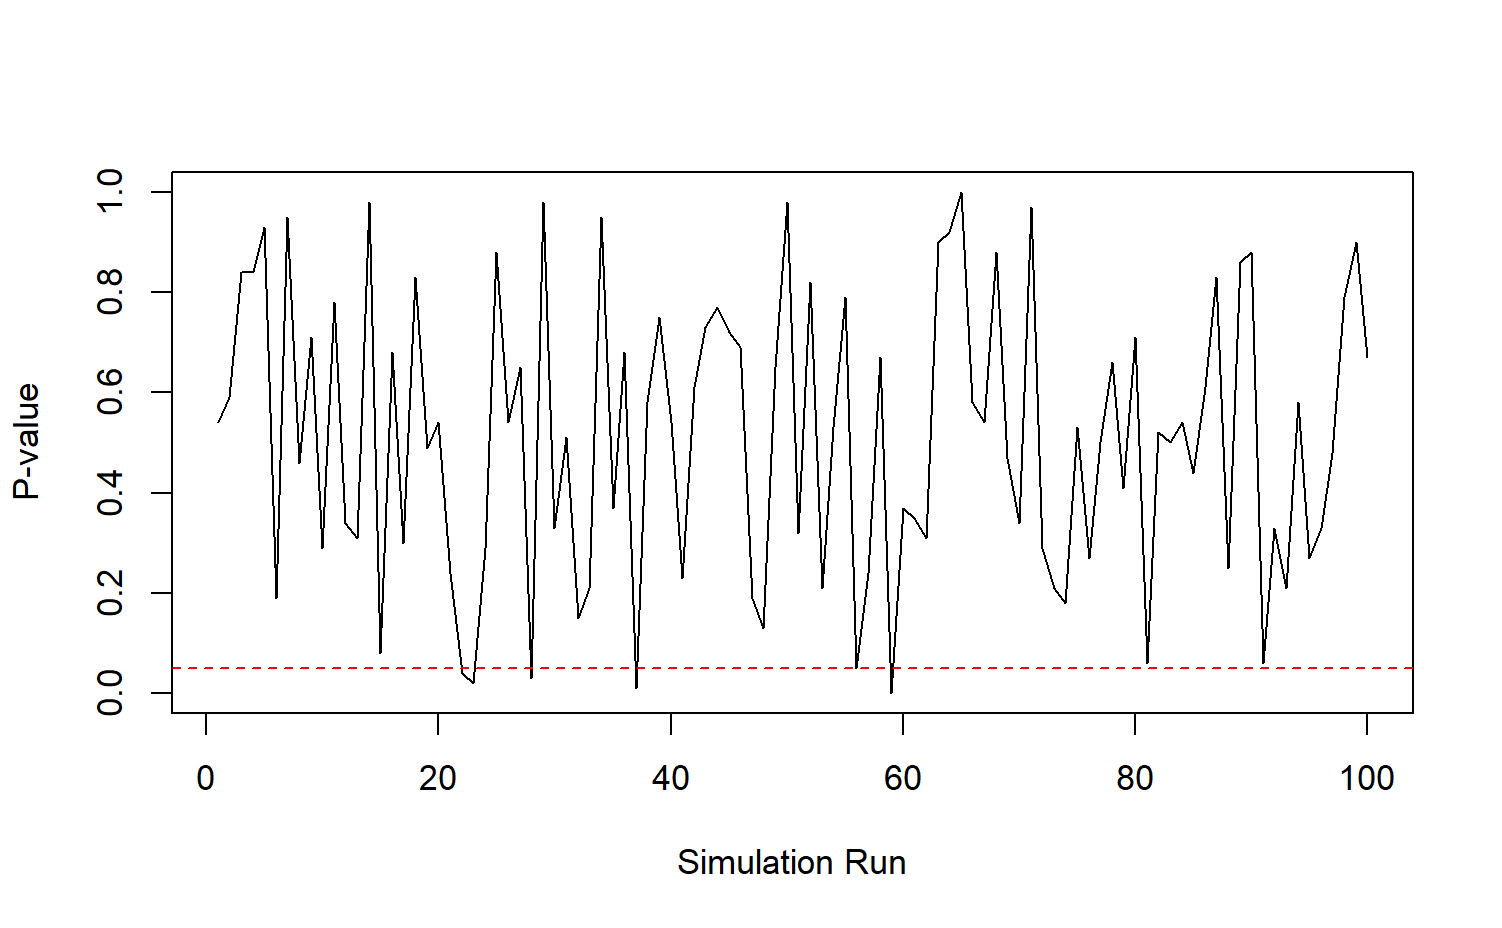
\includegraphics[width=0.4\textwidth]{monte_normal.png}
    }
    \subfigure[Normal v.s. Right-skewed Normal]{        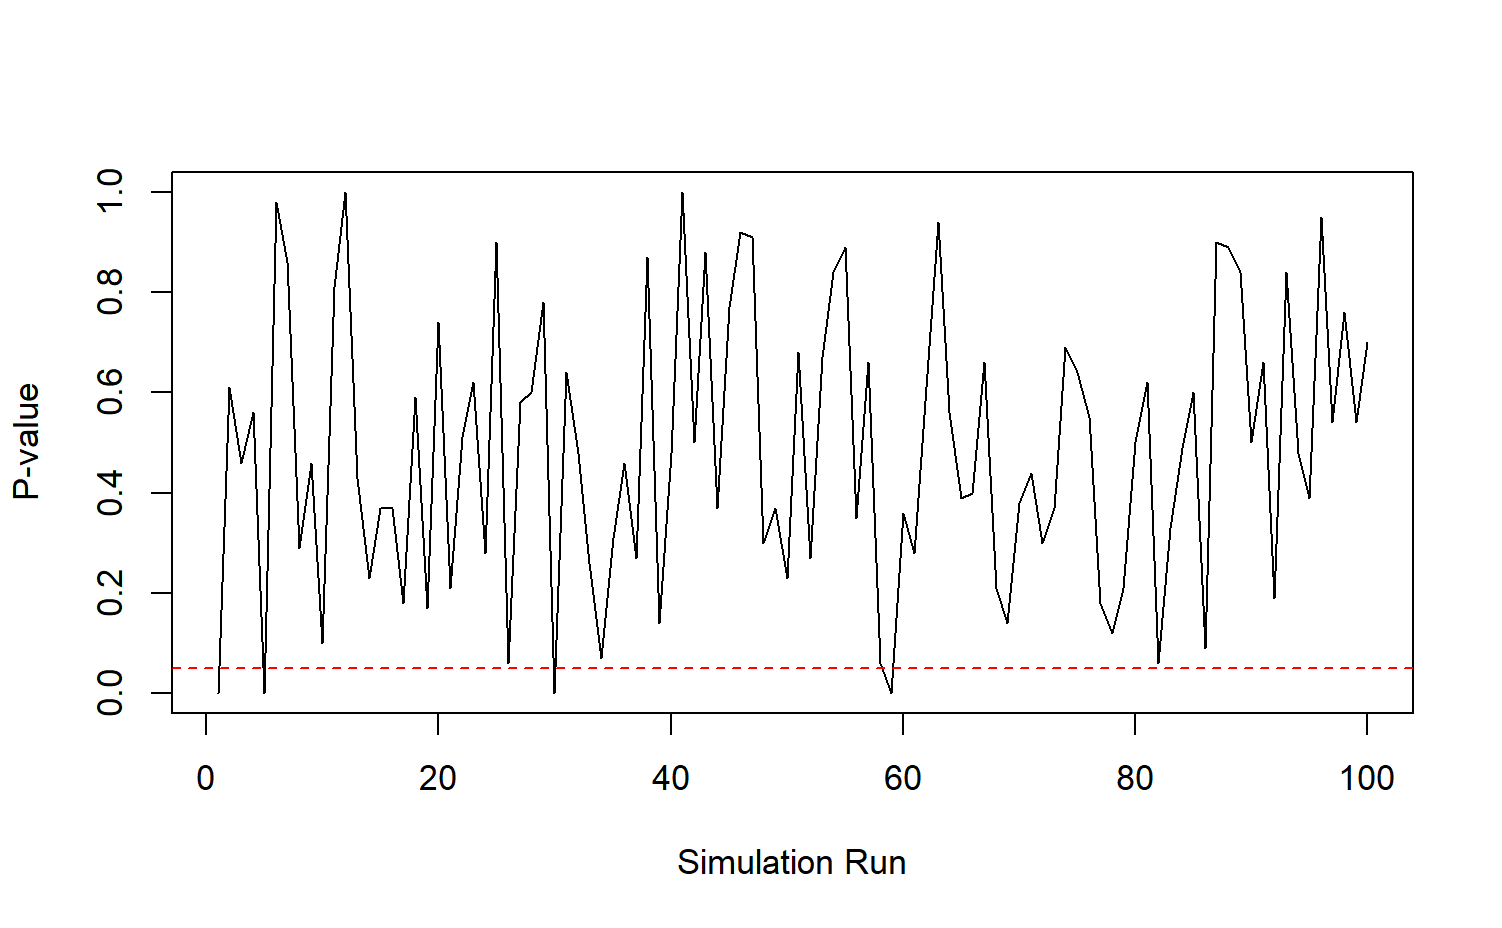
\includegraphics[width=0.4\textwidth]{monte_skewed.png}
    }
    \subfigure[Normal v.s. Exponential]{        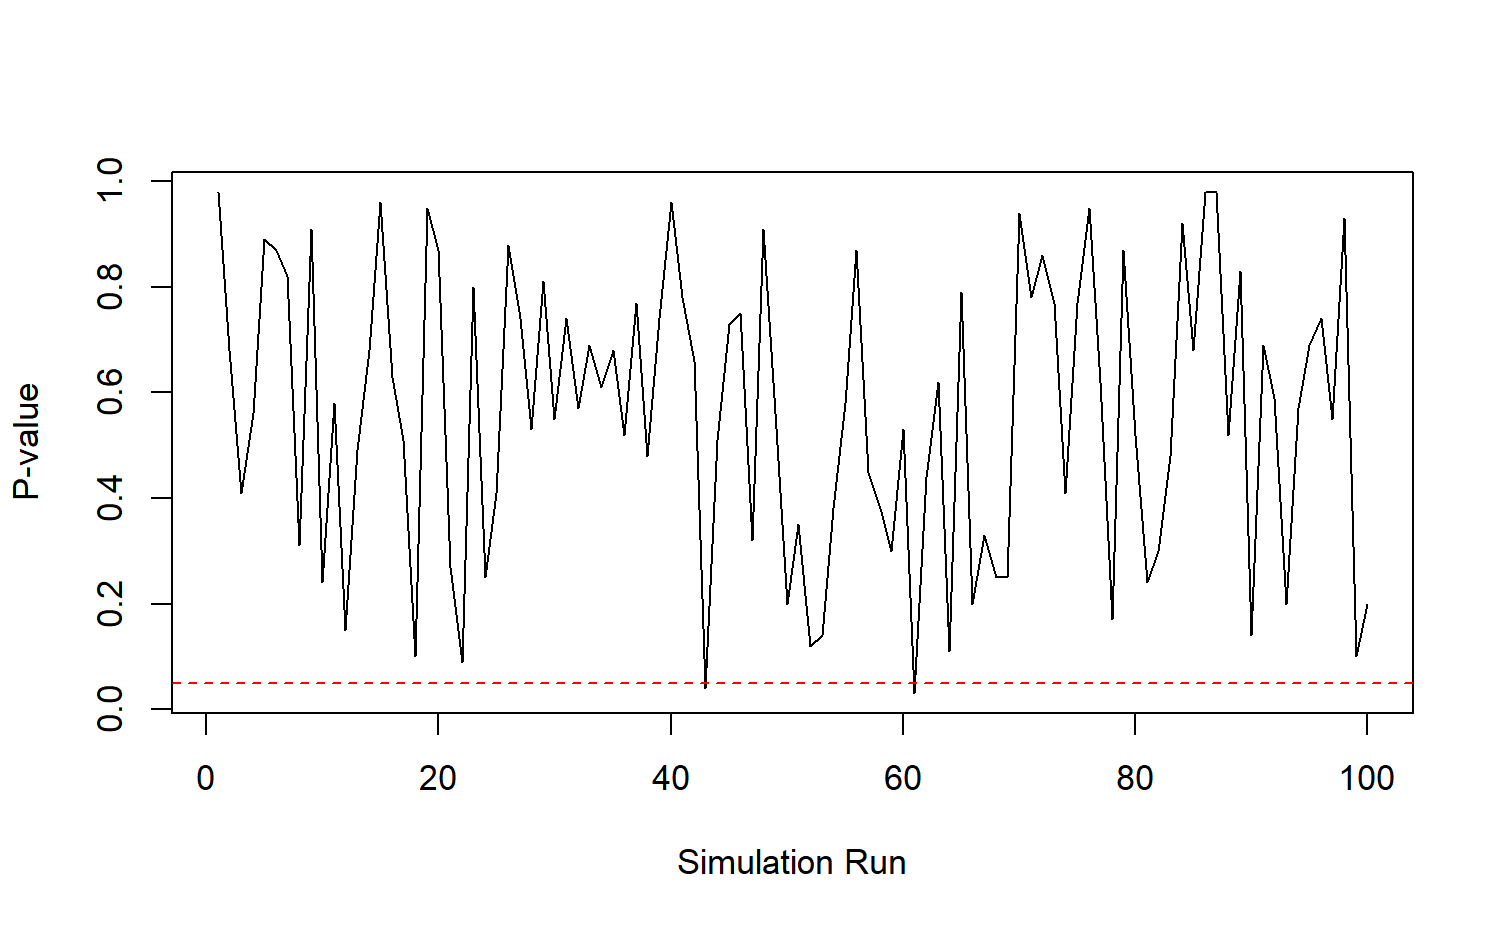
\includegraphics[width=0.4\textwidth]{monte_exp.png}
    }
    \subfigure[Uniform v.s. Uniform]{
        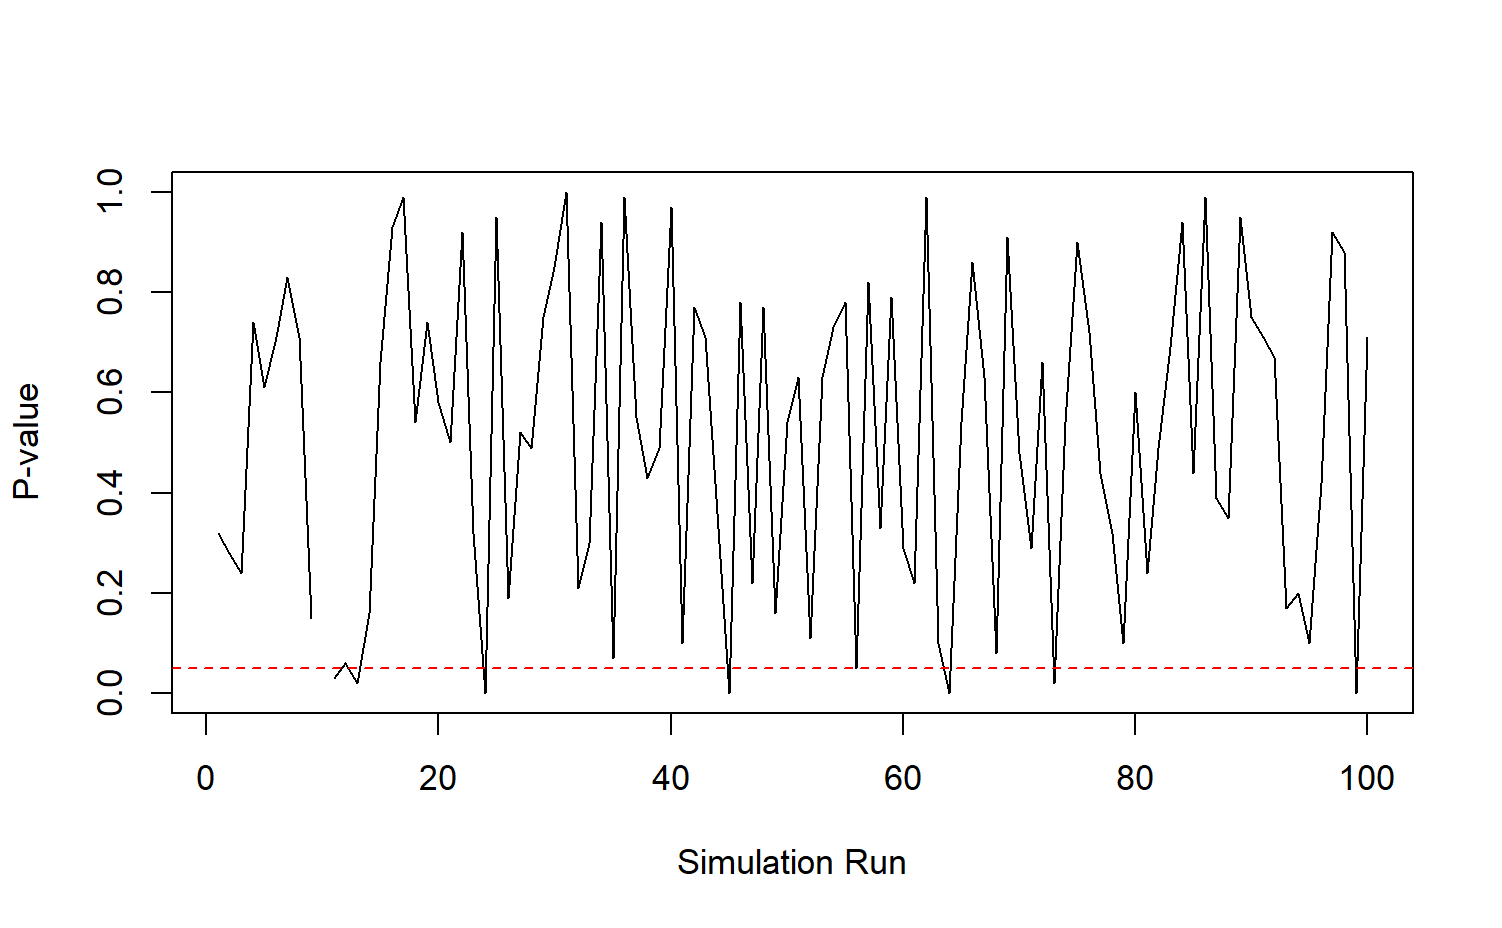
\includegraphics[width=0.4\textwidth]{monte_unif.png}
    }
    \caption{p-values of the Simulation Results}
    \label{4.2}
\end{figure}

From the simulation, we notice that uniform distribution has the most chance of having p-values less than or equal to 0.05. Normal distribution and right-skewed normal distribution have similar chances of having p-values less than or equal to 0.05. While exponential distribution has the least chance of having p-values less than or equal to 0.05. So we should better use this method when data sets are of normal distribution, right-skewed distribution or uniform distribution.


\subsection{Linear Regression}
In this part, we generate data to demonstrate the performance of ordinary least squares (OLS) linear regression under various assumption scenarios.

% Methodology
We simulate three kind of datasets:
\begin{itemize}
    \item Data satisfying the assumptions of linear regression.
    \item Data exhibiting nonlinearity.
    \item Data exhibiting heteroskedasticity.
\end{itemize}

For each dataset, we generate 100 observations. The independent variable x is drawn from a normal distribution with a mean of 50 and a standard deviation of 10. The dependent variable y is constructed differently for each dataset to reflect the respective assumption or its violation.

% Simulation 1: Satisfying Linear Regression Assumptions
For data of the first kind, We create a linear relationship between x and y with normally distributed errors. The linear model's performance is analyzed, with expectations that the OLS estimator will provide unbiased, efficient, and consistent estimates.

% % Operating Characteristics:
% Bias: Expected to be negligible as OLS is BLUE (Best Linear Unbiased Estimator) under Gauss-Markov theorem.
% Mean Squared Error (MSE): Expected to be minimal, reflecting the efficiency of the estimator.
% Confidence Interval Coverage: Expected to be accurate, with 95\% of intervals containing the true parameter value.

% Simulation 2: Nonlinearity
For data of the second kind, y is generated as a function of $x^2$ to introduce nonlinearity. The OLS estimator's bias and inefficiency in the presence of nonlinearity are investigated.

% % Operating Characteristics:
% Bias: Expected to increase due to model misspecification.
% MSE: Expected to be higher than in Simulation 1.
% Type I Error: Investigated by testing the null hypothesis that the coefficient of x is zero.

% Simulation 3: Heteroskedasticity
For data of the third kind, we simulate heteroskedastic errors by making the error variance proportional to x. This setup examines the robustness of OLS estimates to heteroskedasticity.

\begin{figure}[H]
    \centering
    \subfigure[satisfy assumptions]{
        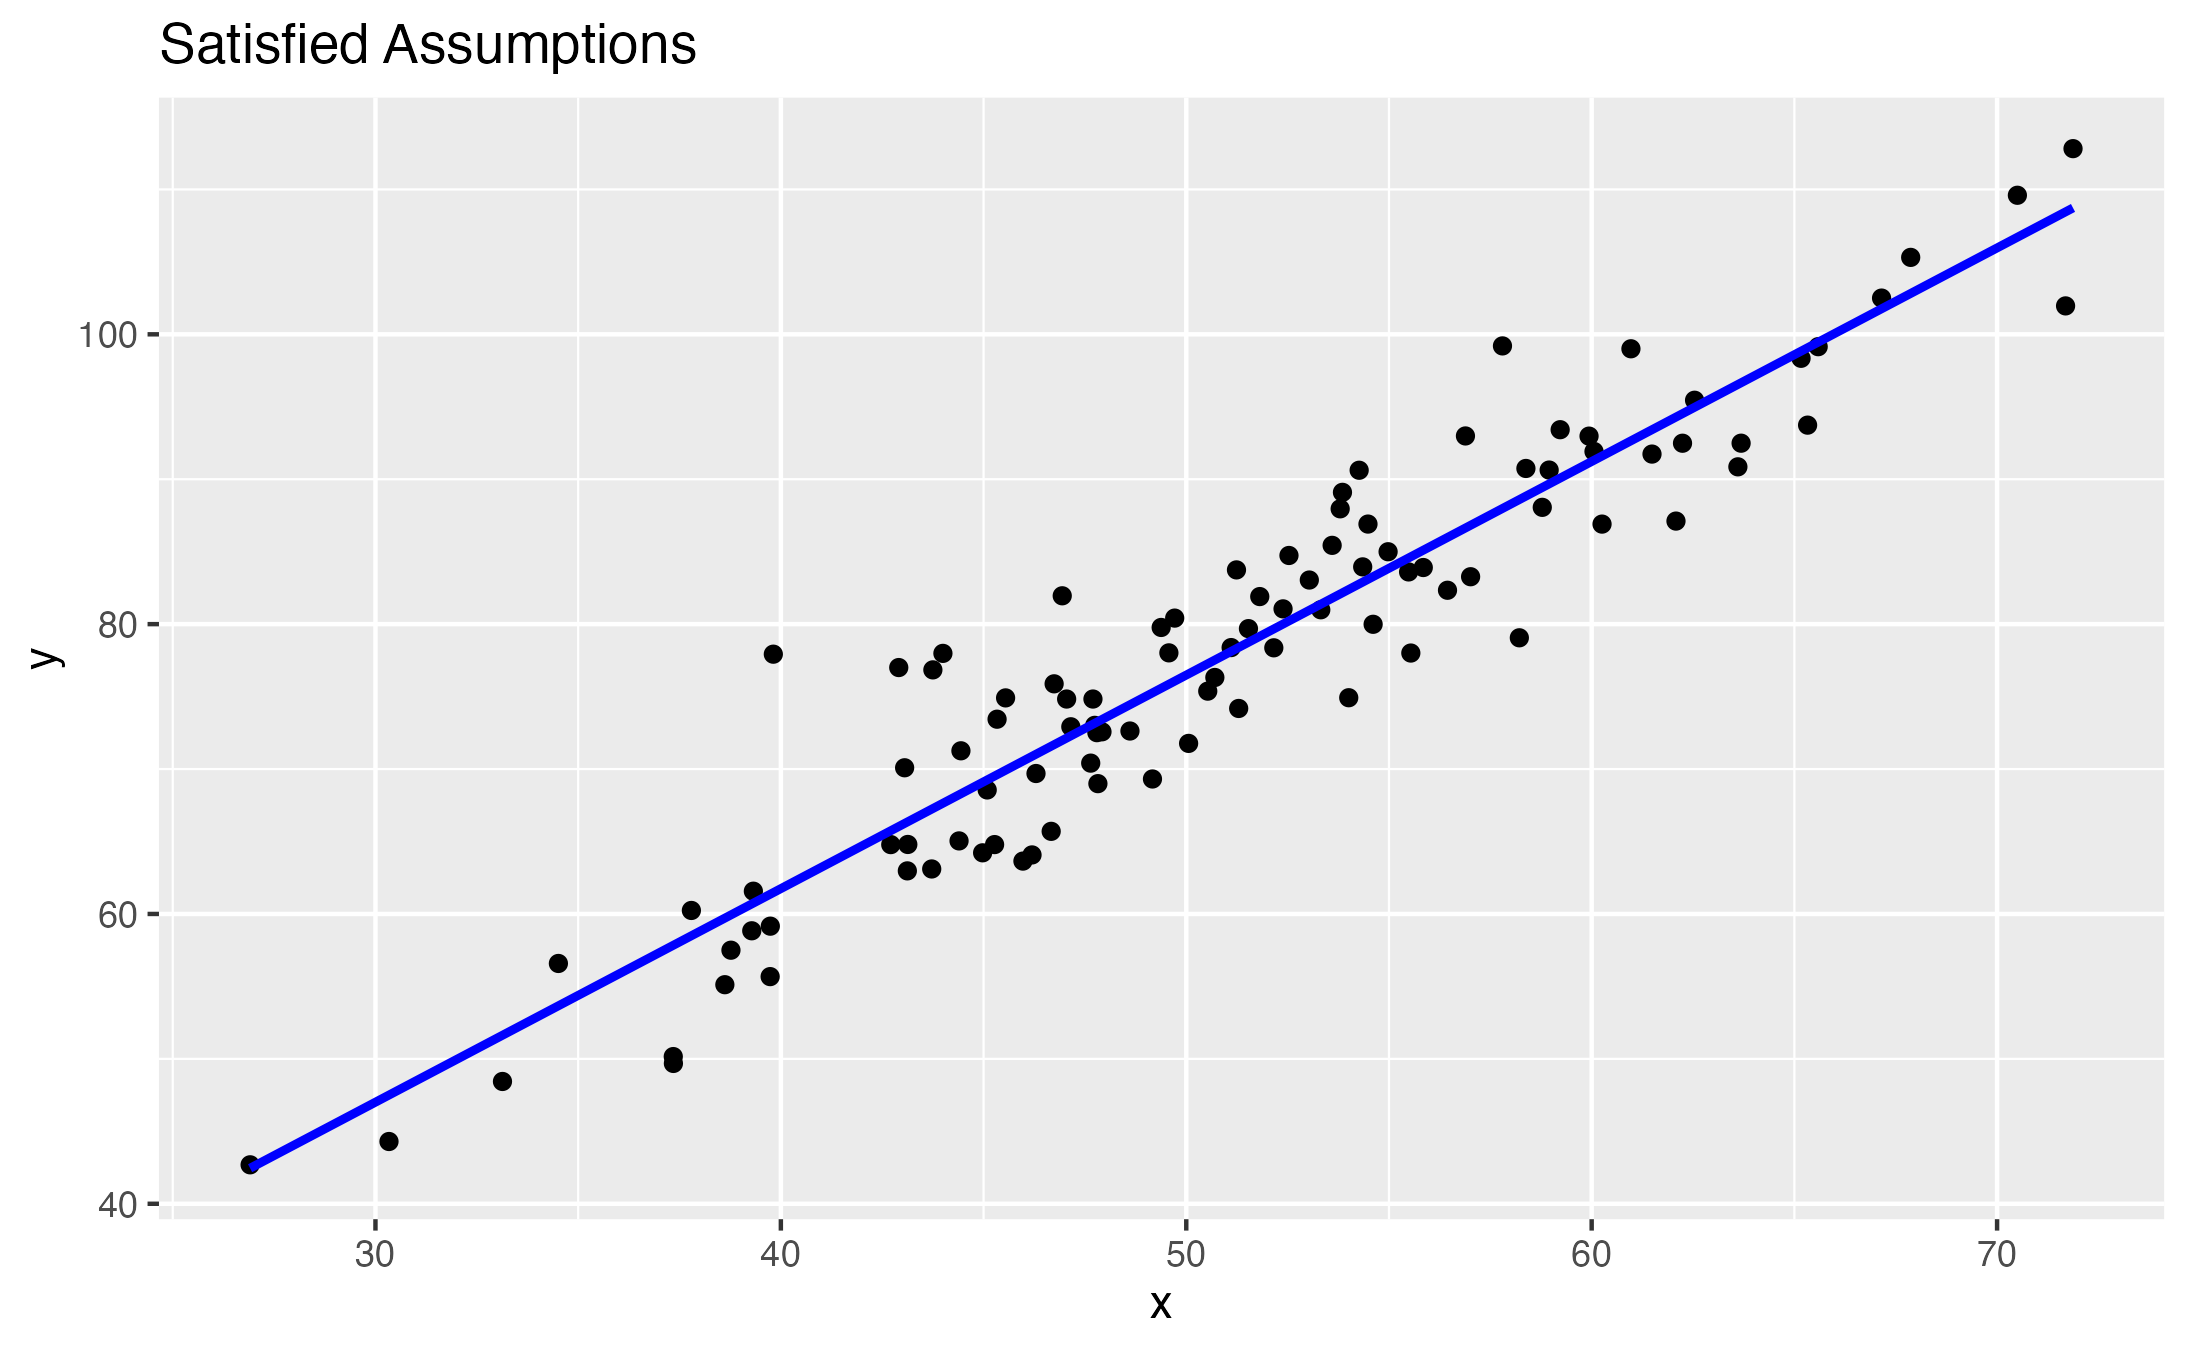
\includegraphics[width=0.3\textwidth]{satisfied_assumptions.png}
        \label{fig:satisfied_assumptions}
    }
    \subfigure[nonlinearity]{
        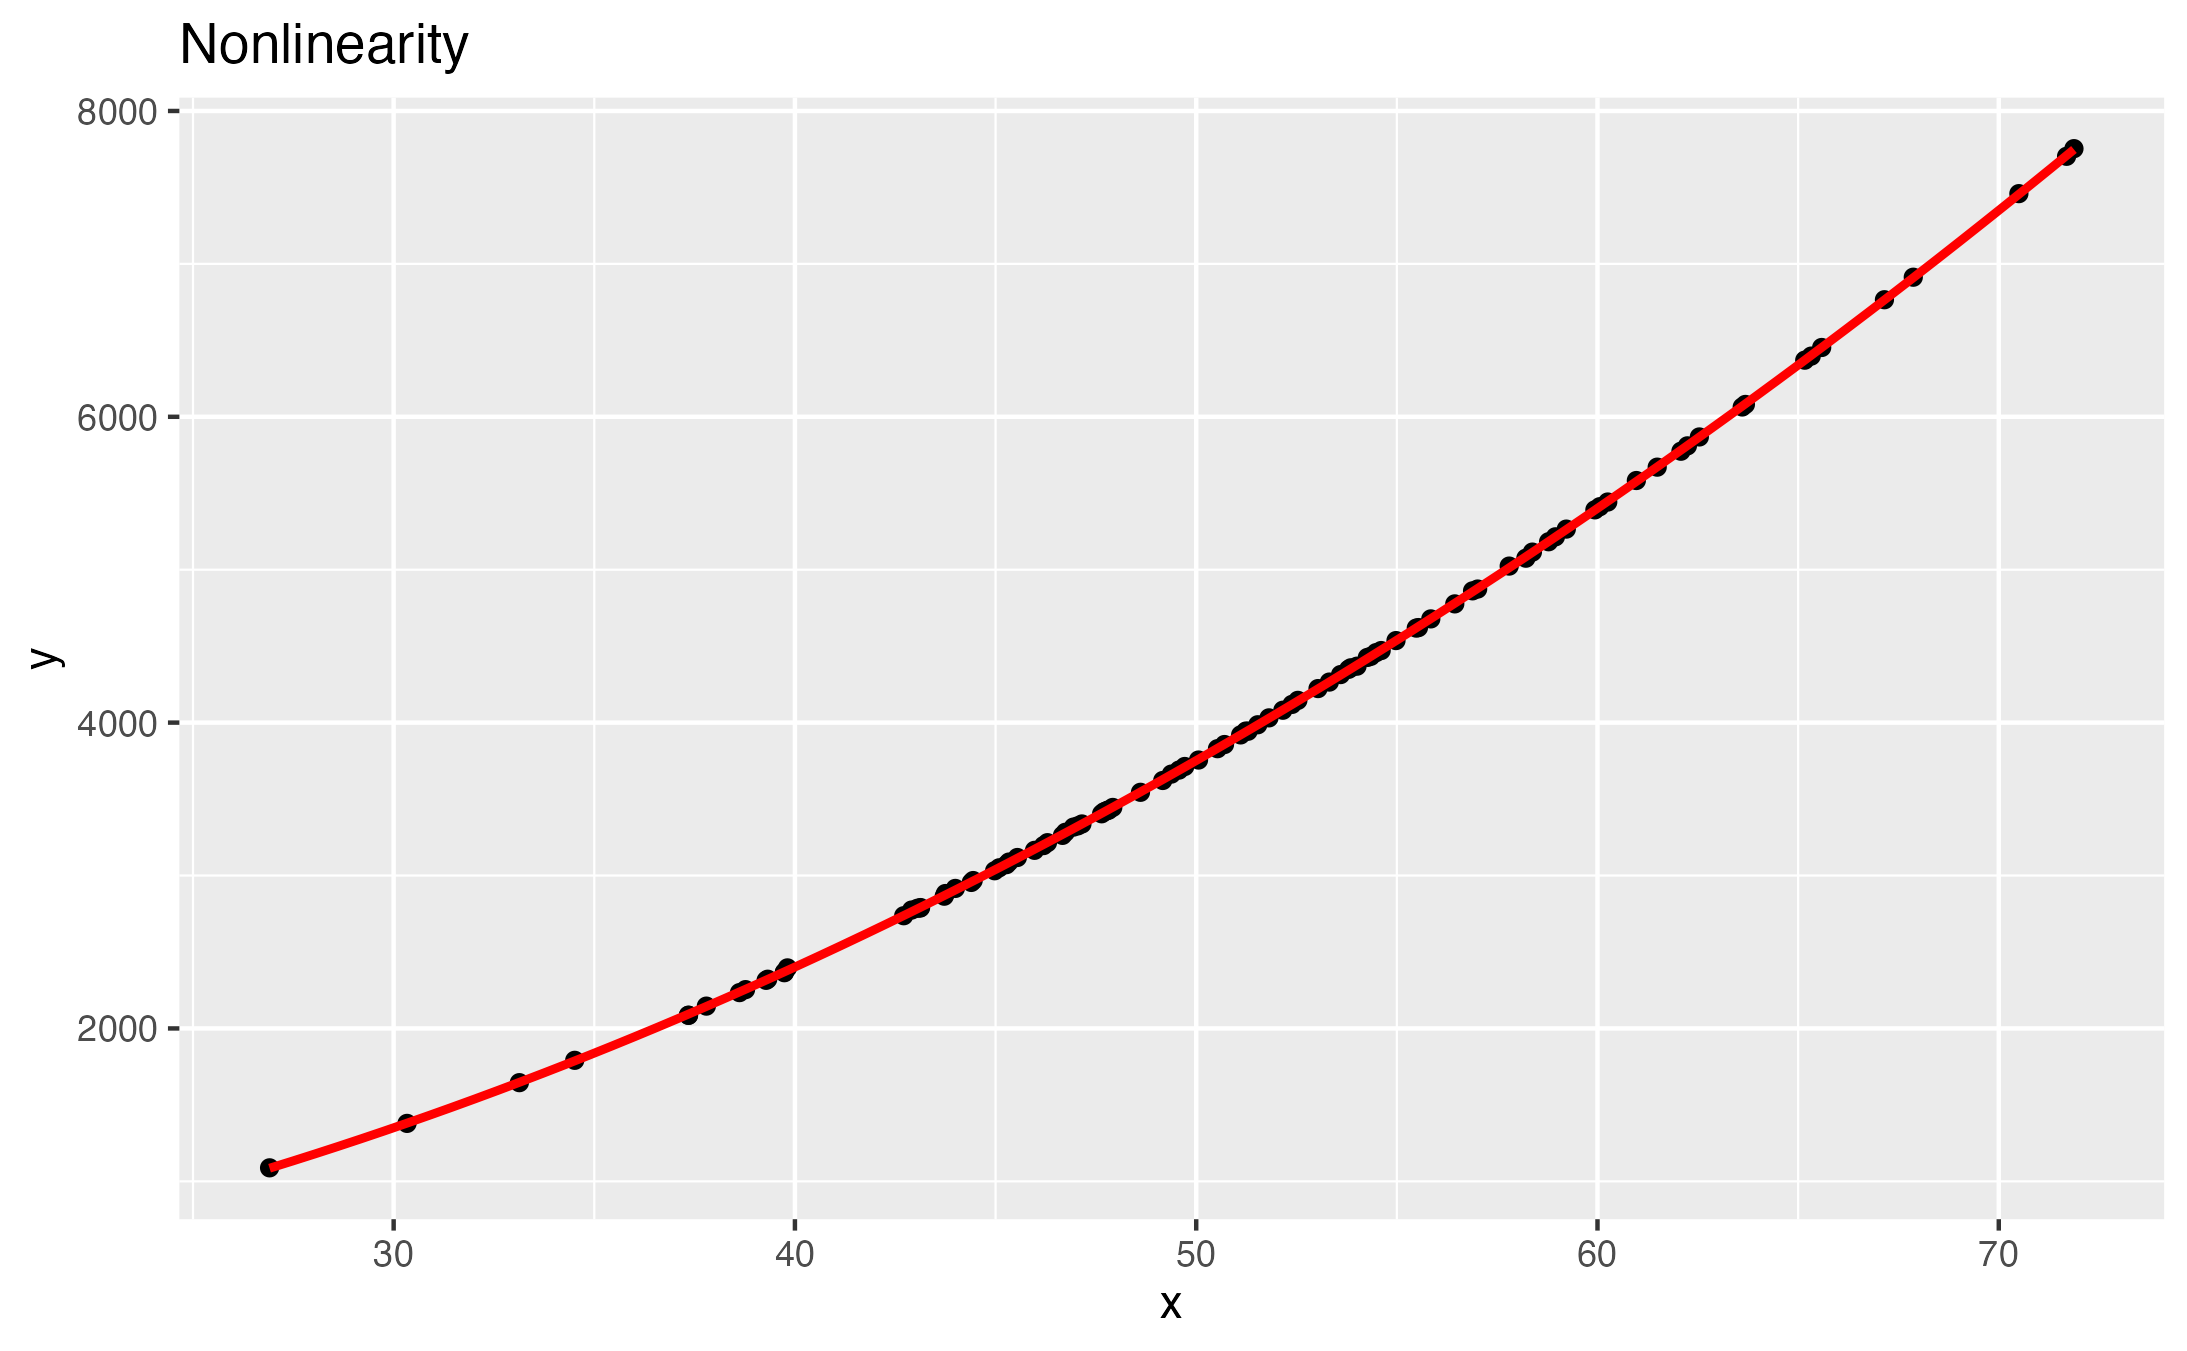
\includegraphics[width=0.3\textwidth]{nonlinearity.png}
        \label{fig:nonlinearity}
    }
    \subfigure[heteroskedasticity]{
        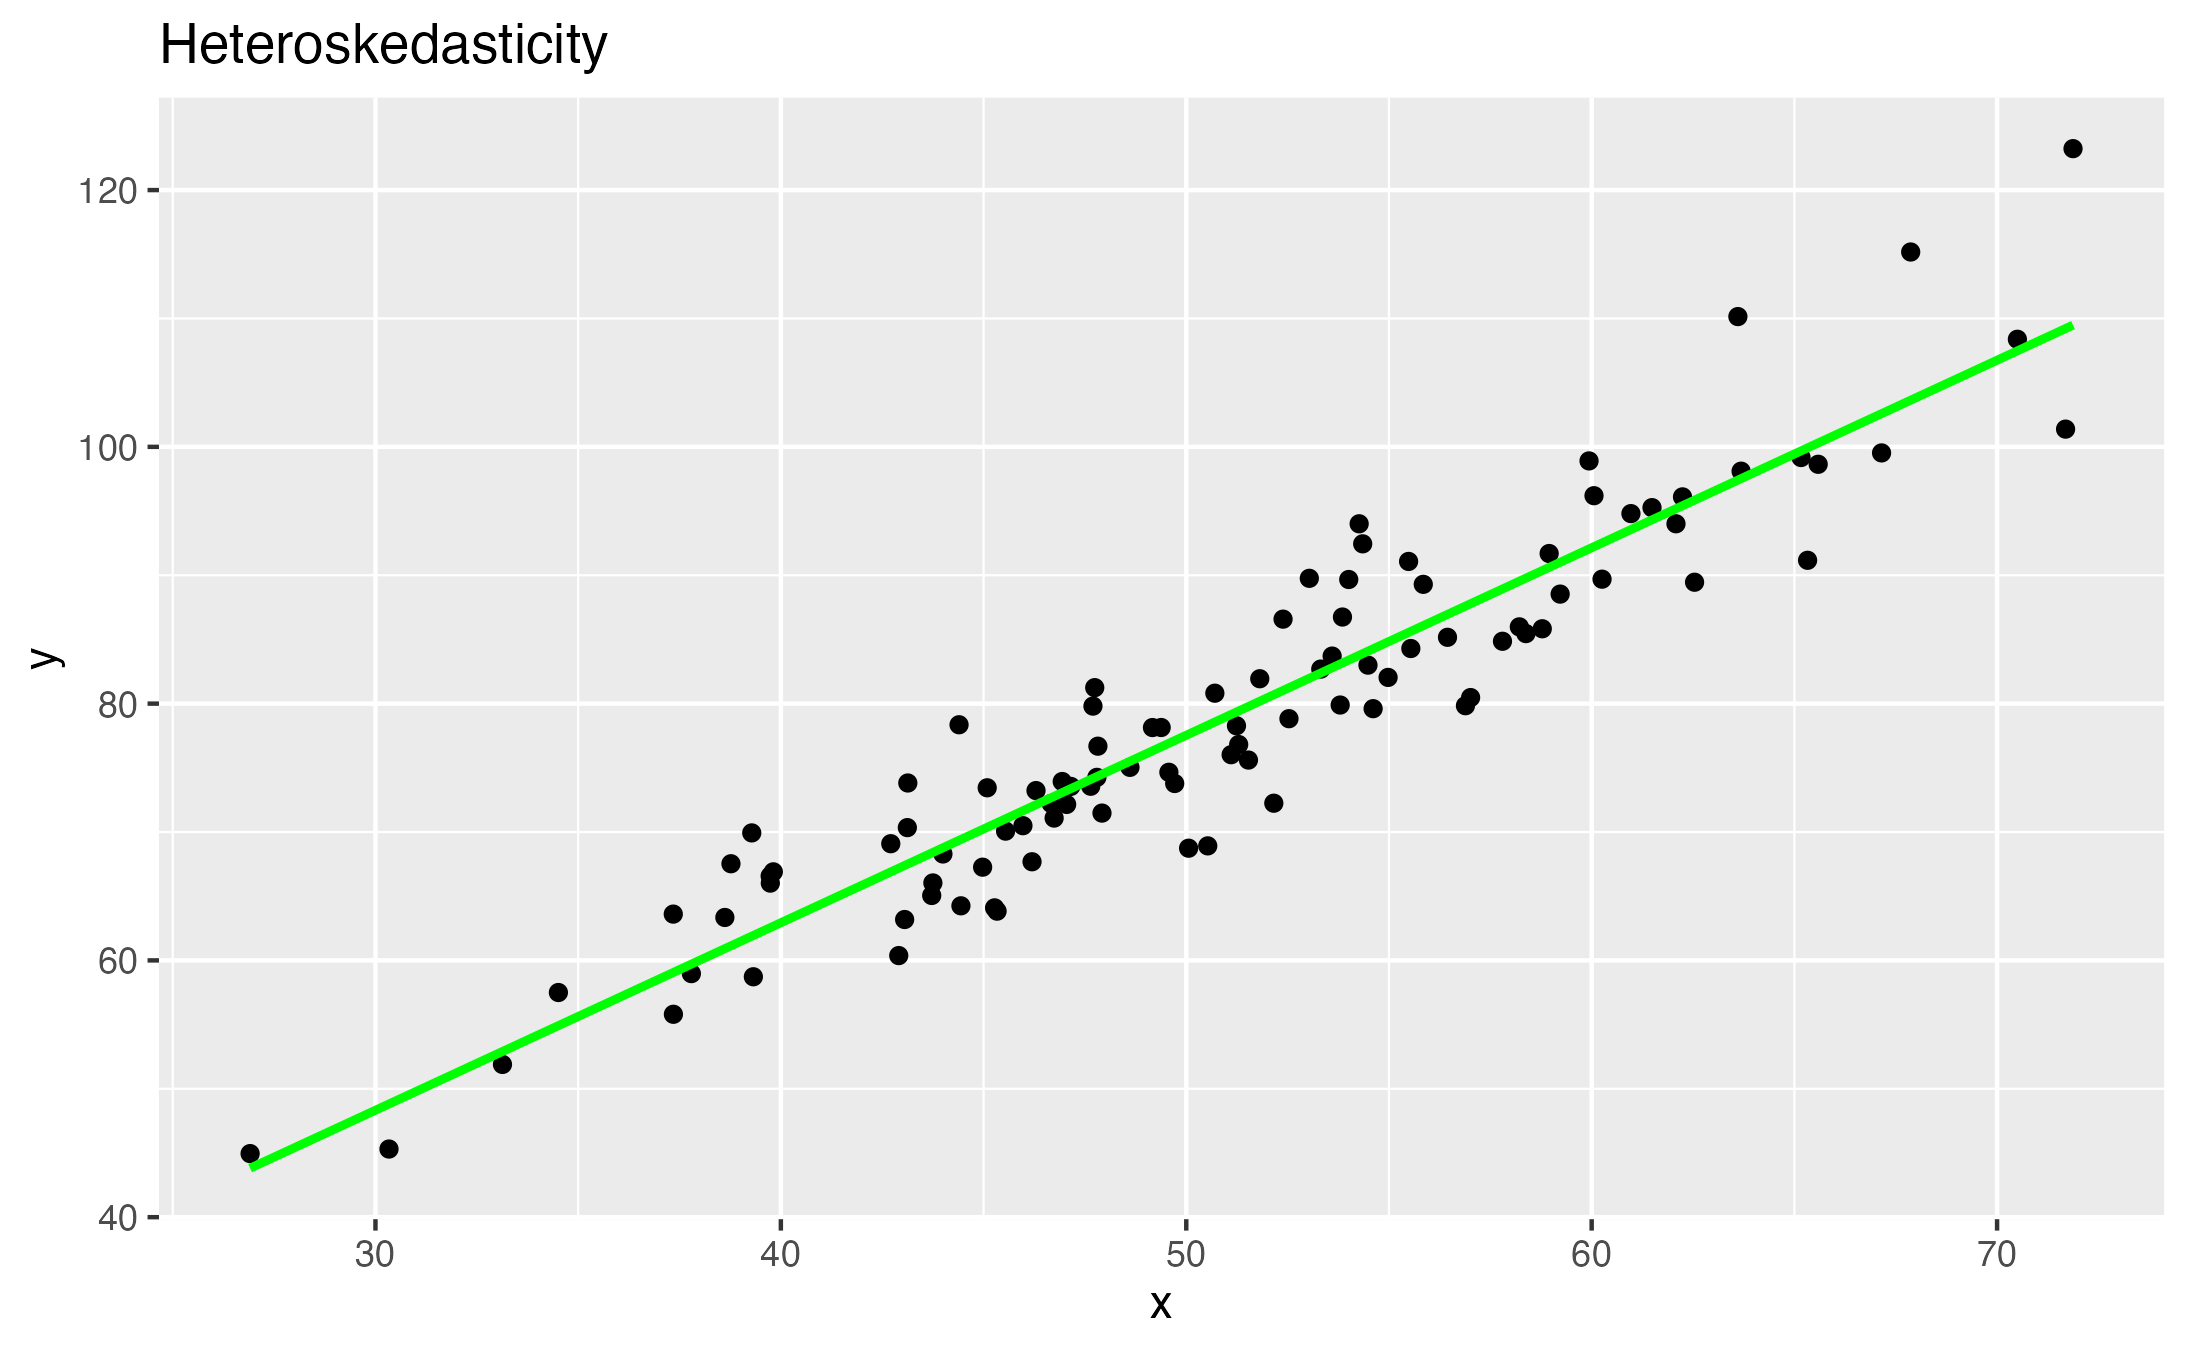
\includegraphics[width=0.3\textwidth]{heteroskedasticity.png}
        \label{fig:heteroskedasticity}
    }
    \caption{Three Mode of the Simulation Results of the Linear Regression}
    \label{fig:lm}
\end{figure}

In our simulations designed to test linear regression under varying conditions, we anticipate distinct outcomes. In the nonlinearity scenario, we expect the linear model to exhibit biased estimates and increased error, highlighting its limitations in capturing complex relationships. In the presence of heteroskedasticity, while coefficient estimates may remain unbiased, the standard errors are likely to be misestimated, leading to unreliable statistical inferences. 

In evaluating the operating characteristics of our three simulations, Mean Squared Error (MSE) serves as a critical metric. For the first simulation, where the data adhere to the assumptions of linear regression, the Residual Standard Error (RSE) is 4.854, translating to an MSE of approximately 23.561. This relatively low MSE aligns with our expectation that the OLS estimator. 

In the second simulation, which introduces nonlinearity, the RSE is marginally lower at 4.852, leading to a similar MSE. Despite the small difference in MSE from the first simulation, this result might be deceptive. The non-linear relationship between variables is expected to increase bias due to model misspecification, which is not directly captured by MSE but can significantly impact the model's predictive accuracy and reliability.

The third simulation, featuring heteroskedastic errors, shows a slightly higher RSE of 4.901. This results in an MSE of approximately 24.020, slightly higher than in the previous simulations. This increase in MSE is in line with our hypothesis that heteroskedasticity, where error variances vary with the level of the independent variable, can reduce the efficiency of OLS estimates. 

These MSE values underscore the importance of considering such violations in real-world data analysis, as they can subtly yet significantly impact the performance of the OLS estimator. In the later analysis, we should take into consideration whether it displays a non-linearity mode and heteroskedasticity pattern. If this is the case, we should take more care of this model. 

% % Operating Characteristics:
% Bias: Remains unbiased, as OLS estimates are not affected by heteroskedasticity in terms of bias.
% MSE: Expected to increase, reflecting the loss of efficiency.
% Confidence Interval Coverage: May be compromised, as standard errors are typically underestimated in the presence of heteroskedasticity.
% Visualization
% Each simulation's results are visualized using scatter plots with regression lines. These plots provide a clear representation of the data's adherence to or deviation from the assumptions.

% % Analysis of Results
% The bias, MSE, and other characteristics are computed for each simulation to quantitatively assess the performance of the OLS estimator under each condition.

% % Computational Efficiency
% The computational time for each simulation is recorded to compare the efficiency of the OLS estimator across different scenarios.

% % Discussion
% The simulations illustrate the importance of assumption checking in linear regression analysis. While OLS performs optimally when assumptions are met, violations such as nonlinearity and heteroskedasticity can lead to inefficiencies and unreliable inference. These findings underscore the necessity of exploratory data analysis and diagnostic checking in practice.

% % Conclusion
% The simulations demonstrate the OLS estimator's strengths and limitations. When the linear model assumptions are satisfied, the estimator performs well, but when these assumptions are violated, the performance deteriorates. This reinforces the need for robust or alternative methods in the presence of assumption violations.

\section{Analysis}

 In this part, we will firstly examine the real data to make sure it agrees with each method's assumption. Then, we will use the method to explore the relationship between school shooting injuries and other feature.

\subsection{Welch’s permutation t-test}

We inspect each binary feature in our dataset by firstly drawing its density plot and determine its shape. Then, we perform Welch’s permutation t-test to obtain its p-value. If p-value is smaller than 0.05, a traditional statistical bound, we can safely draw the conclusion that this feature will affect school shooting injuries number.

\begin{table}[H]
\centering
\begin{tabular}{|c|c|c|}
\hline
Feature Name                        & Distribution & P-value                       \\ \hline
Shooter's Gender (Male/Female)      & Normal       & 0.336                         \\ \hline
Shooter's Race (White/Black)        & Normal       & 0.334                         \\ \hline
Shooter's Bullied Experience (Y/N)  & Right-skewed & 0.087                         \\ \hline
Shooter's Domestic Violence (Y/N)   & Normal       & 0.878                         \\ \hline
Preplanned (Y/N)                    & Right-skewed & 0.01  
\\ \hline
During School Day (Y/N)             & Normal       & 0.025 
\\ \hline
During Sports (Y/N)                 & Normal       & 0.581                         \\ \hline
During School Sponsored Event (Y/N) & Normal       & 0.783                         \\ \hline
\end{tabular}
\caption{Welch’s permutation t-test results on features}
\label{perm_result_table}
\end{table}

From the results presented in Table \ref{perm_result_table}, we observe varying impacts of different features. Notably, the "During School Day" feature not only adheres to our assumption of a normal or left-skewed normal distribution but also exhibits a p-value of 0.025, which is below the traditional significance threshold of 0.05. This suggests that the occurrence of school shootings during school hours significantly influences the number of injuries. It is also worth mentioning that although the p-value for "Preplanned" is only 0.01, we cannot take this into account because it violates our assumption as it is "Right-skewed". This finding is of particular interest as it highlights a specific context in which school shootings are more consequential in terms of injuries.

In contrast, other features such as "Shooter's Gender," "Shooter's Race," and "Shooter's Domestic Violence" show p-values much higher than 0.05, indicating that we cannot confidently assert their statistical significance in relation to school shooting injuries based on our current analysis. Additionally, some features like "Shooter's Bullied Experience" is characterized by right-skewed distributions, which may necessitate different analytical approaches.

The results lead us to a nuanced understanding of the factors influencing school shooting injuries. While certain features like "During School Day" are statistically significant, others may require further investigation using alternative methods. This comprehensive approach ensures a thorough and informed analysis of the factors contributing to school shooting injuries. In the following section, we will explore additional methods to assess the impact of features that did not show significance in the Welch’s permutation t-test, thereby ensuring a holistic examination of all potential influences.

\subsection{Monte Carlo Hypothesis Testing}

We work on numeric predictors of real data in this section. Firstly, we look at the distribution of our response and other numeric predictors. Then we perform Monte Carlo Hypothesis Testing on linear correlation between our response and numeric predictors. If the p-value is smaller than 0.05, which is the significance level defined by us in previous sections, we can safely reach the conclusion that the predictor has linear relationship with our response.

Table \ref{tb2} provides all p-values of numeric predictors from Monte Carlo Hypothesis Test. According to this table, we notice that "Reliability Score", "Wounded" and "Shooter's Age" have significantly small p-values. Their distributions also agree with the simulation results, that we should apply Monte Carlo Hypothesis Test when data sets are of normal distribution and right-skewed distribution. We can conclude that "Reliability Score", "Wounded" and "Shooter's Age" will have linear relationship with the total killed and injured peopler in school shooting.

\begin{table}[H]
\centering
\begin{tabular}{|c|c|c|}
\hline
Feature Name                        & Distribution & P-value                       \\ \hline
Reliability Score (1-5)     & Normal       & 0.00                             \\ \hline
Killed Includes Shooter        & Bimodal       & 0.02                       \\ \hline
Wounded     & Right-skewed      & 0.00                        \\ \hline
Victim's Ages   & Right-skewed       & 0.28                        \\ \hline
Duration Minutes                    & Right-skewed & 0.99 
\\ \hline
Number of Shots Fired             & Right-skewed      & 0.35\\ \hline
Number of Shooters                 & Right-skewed       & 1.00\\ \hline
Shooter's Age & Right-skewed       & 0.00                       \\ \hline
\end{tabular}
\caption{P-values of numeric predictors from Monte Carlo Hypothesis Test}
\label{tb2}
\end{table}


\subsection{Linear Regression}

We would like to predict the number of injuries each school shooting incidence. Having inspected the data, we noticed that some features are numerical and some are categorical. Since we have shown the importance of linearity and non-heteroskedasticity in simulation part, we will check the two properties before applying linear regression. 

To be more specific, we check linearity by visual inspection using plot function in R. With respect to categorical features, a noticeable and consistent difference in the patterns across categories can be an indication that x is a good predictor for y. For non-heteroskedasticity, we observe how the variability of injuries varies across the levels of  categorical predictor variables.

\subsubsection{Categorical Features}

\begin{figure}[H]
    \centering
    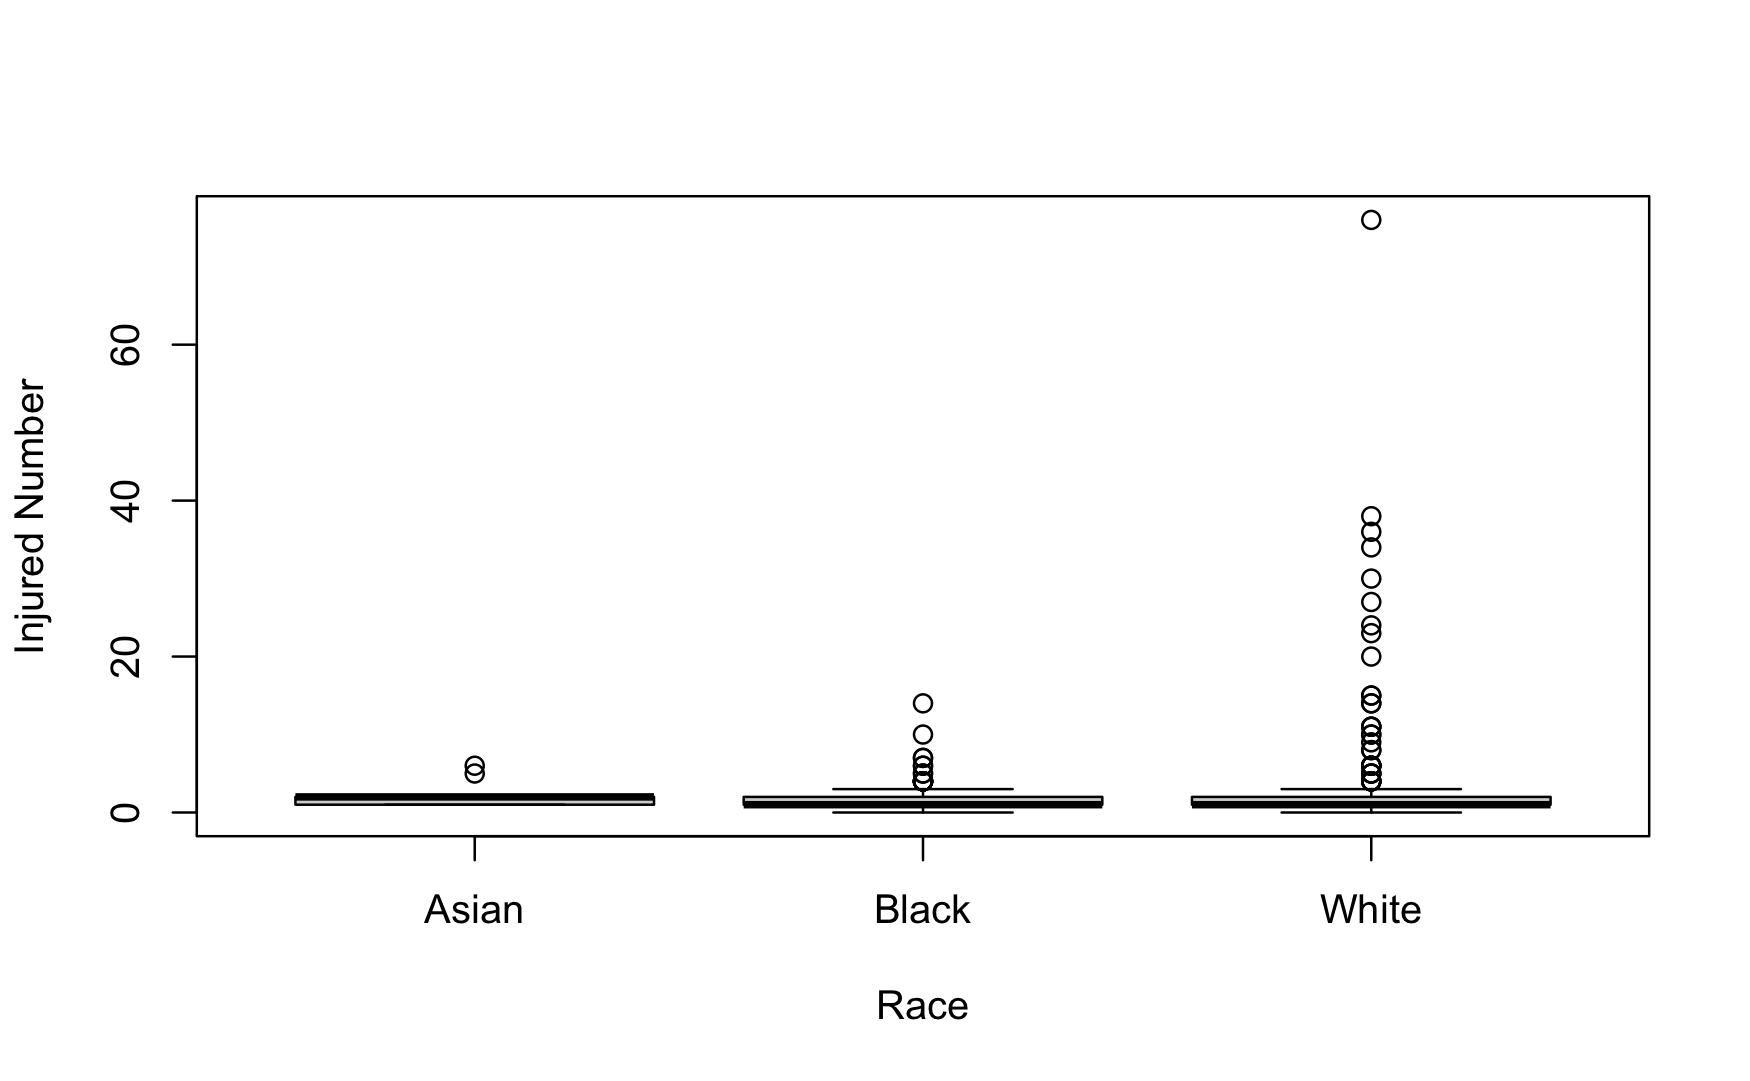
\includegraphics[width=0.8\textwidth]{lm_race_box.png}
    \caption{Box plot between shooter's race and number of injuries}
    \label{lm_race_box}
\end{figure}

Among categorical features, we find that pre-planned, shooting category, firearm type show a clear pattern in different types. Take \ref{lm_race_box} as an example, the graph indicates that shooter with white race is likely to cause more injuries. However, the variance of injuries with white shooter is evidently higher than those with asian and black shooters. Based on the inference from graphs, we may not continue to perform linear regression between this feature and injuries. 

We repeat this process to other categorical variables. Note that we transform categorical features into dummy variables, and use lm model to see coefficient for different categories.

The table below summarizes the relationships between various categorical features and the number of injuries in school shootings. These relationships are identified based on the patterns observed in our data analysis, where we transformed categorical features into dummy variables and assessed them using linear regression models.

\begin{table}[H]
\begin{tabular}{|c|c|c|}
\hline
Feature Name & Positive Relationship with Injuries & Negative Relationship with Injuries \\ \hline
Category     & Illegal Drug Related, Gang-related  & Accidental, Suicide/Attempted       \\ \hline
Firearm Type & Rifle, Shotgun                      & Handgun                             \\ \hline
Race         & White                               & Black, Asian                        \\ \hline
\end{tabular}
\label{lm_cate_results}
\end{table}

For instance, in the 'Category' feature, incidents related to illegal drugs and gang activities show a positive correlation with the number of injuries, suggesting a higher injury count in these scenarios. Conversely, accidental incidents and suicides or attempted suicides are associated with fewer injuries.

Regarding 'Firearm Type,' the use of rifles and shotguns is positively associated with the number of injuries, indicating that these types of firearms are more likely to result in higher injury counts compared to handguns.

Finally, the 'Race' feature reveals a complex and sensitive pattern. It shows that incidents involving white shooters are associated with a higher number of injuries compared to those involving black or Asian shooters. This finding is significant as it challenges common stereotypes and emphasizes the need for a nuanced understanding of the factors influencing the severity of school shootings.

\subsubsection{Numerical Features}

Among numerical features such as shooter's age, duration, the number of shots, the number of shooters, we only find that the number of shooters shows a linear relationship with injuries with no evidence of heteroskedasticity. Therefore, we perform linear regression on this feature. Results shows that the number of shooters are positively related to injuries, with a coefficient of 0.9705 and strong significance level.

\section{Discussion}

In this study, we conducted an analysis to investigate the relationship between various features and the number of injuries per school shooting incident. We employed Welch's permutation t-test, Monte Carlo hypothesis testing and linear regression to examine these relationships and draw meaningful conclusions. While our analysis yielded valuable insights, it is important to acknowledge the limitations of these statistical methods and the potential impact on our findings.

\subsection{Welch's Permutation T-test}

In summary, Welch's Permutation T-test is a strong method in figuring out categorical data that has a non-trivial impact on injuries per school shooting. However, we cannot ignore the restrictions due to the nature of this method.

The primary limitations of Welch's permutation t-test is its binary feature requirement. This method is suitable for comparing features with two distinct categories, making it less applicable when dealing with categorical variables with multiple levels. In our study, this limitation forced us to dichotomize some variables, potentially oversimplifying the complexity of the data. 

Additionally Welch's t-test assumes that observations within each category are independent. In the context of school shooting incidents, this assumption may not always hold, as events can be influenced by various external factors that affect multiple incidents simultaneously. Violations of this assumption may lead to inaccurate p-values and effect size estimates.


\subsection{Monte Carlo Hypothesis Testing}
Monte Carlo hypothesis testing is a robust computational approach that can approximate the p-value by simulating the sampling distribution of a test statistic. However, there are several limitations and assumptions inherent in this method that can impact the findings:

1. \textbf{Model Assumptions}: Monte Carlo simulations rely on the correct specification of the model, including the distribution of the data. If the data do not conform to the model assumptions, the results of the hypothesis test can be misleading.

2. \textbf{Dependency Among Observations}: Similar to Welch's t-test, Monte Carlo hypothesis testing assumes that the observations are independent. In the case of school shootings, there could be underlying factors or dependencies between incidents that the test does not account for, such as geographic proximity or time clustering of events.

3. \textbf{Computational Intensity}: Monte Carlo methods can be computationally intensive, requiring a large number of simulations to achieve an accurate estimate of the p-value. This can be particularly challenging with large datasets or complex models.

4. \textbf{Randomness and Reproducibility}: The randomness inherent in Monte Carlo methods means that results can vary from one simulation to another unless a fixed seed is used for random number generation. This can affect the reproducibility and stability of the results.

5. \textbf{Resolution of P-Values}: The resolution of p-values in Monte Carlo hypothesis testing is limited by the number of simulations run. For example, if 10,000 simulations are run, the smallest possible p-value is 1/10,000, which may not be sufficient to detect very small effect sizes.

6. \textbf{Overfitting}: There is a risk of overfitting, especially when multiple hypothesis tests are conducted. Without proper adjustments for multiple comparisons, the probability of finding at least one statistically significant result due to chance increases.


\subsection{Linear Regression}
Linear regression, a key method in our analysis, assumes a linear relationship between independent and dependent variables. However, this assumption can be overly simplistic, as real-world relationships, such as those between various factors and the number of injuries in school shootings, may not always be linear. In our study, we did not extensively explore potential nonlinear relationships, such as by employing feature transformation techniques within our linear models. Furthermore, our approach primarily involved examining each feature individually in relation to injuries, which doesn't capture the potentially intricate interplay among various factors. This singular focus may overlook the complex, multifaceted nature of how different features collectively influence the outcome. Recognizing these limitations highlights the need for more sophisticated models that can account for both nonlinear dynamics and the interaction effects between multiple variables in future research.


\section{Statement of Responsibility}
\begin{itemize}
    \item Beijie Liu: Frame the architecture of project and apply linear regression on simulation and analysis
    \item Xinlei Cai: Compose introduction part and apply Welch's permutation t-test on simulation and analysis
    \item Jingyan Zhang: Make plots for data visualization and apply Monte Carlo hypothesis testing on simulation and analysis
\end{itemize}


\newpage
\nocite{*}
\printbibliography

\end{document}
